
\documentclass{article}

% Required for inserting images
\usepackage{graphicx}

% to have precise image placement
\usepackage{float}

% to insert hiperlinks
\usepackage[colorlinks=true,linkcolor=cyan]{hyperref}

% to have better references
\usepackage[nameinlink]{cleveref} 

%\usepackage[noabbrev]{cleveref}

% to use prefix for references
\usepackage{etoolbox}

% to set the margin of the page
\usepackage[a4paper, left=25mm,top=20mm,bottom=20mm,right=15mm]{geomet ry}

% to make indentations
\usepackage{changepage}

% for sub figures
\usepackage{subcaption}

% to allow putting description text to te side of an image
\usepackage{wrapfig}

\usepackage{multirow}

% for the table
\usepackage[table,xcdraw]{xcolor}

% code highlighter
\usepackage{listings}

\usepackage{color}

% To have a paragraph look like a subsubsubsection
\usepackage{titlesec}

\setcounter{secnumdepth}{4}

\titleformat{\paragraph}
{\normalfont\normalsize\bfseries}{\theparagraph}{1em}{}
\titlespacing*{\paragraph}
{0pt}{3.25ex plus 1ex minus .2ex}{1.5ex plus .2ex}


\definecolor{dkgreen}{rgb}{0,0.6,0}
\definecolor{gray}{rgb}{0.5,0.5,0.5}
\definecolor{mauve}{rgb}{0.58,0,0.82}
\definecolor{orage}{rgb}{0,0.26,0.99}

\lstset{frame=tb,
  language=python,
  aboveskip=3mm,
  belowskip=3mm,
  showstringspaces=false,
  columns=flexible,
  basicstyle={\small\ttfamily},
  numbers=none,
  numberstyle=\tiny\color{orage},
  keywordstyle=\color{blue},
  commentstyle=\color{dkgreen},
  stringstyle=\color{mauve},
  breaklines=true,
  breakatwhitespace=true,
  tabsize=3
}

% to include svg images
%\usepackage{svg}

% settings for how to indent the page when needed
\newenvironment{indented_section}
  {\adjustwidth{3em}{0pt}}
  {\endadjustwidth}

 \title{Use Of Jigsaw Puzzle Solving Algorithms In The Real World}
 \author{Luca Sartore}
 \date{May 2023}



\begin{document}

% \maketitle

\begin{center}

  
\includegraphics[scale=1]{pictures/unitn_logo.pdf}

  \vspace{2 cm} 

  \LARGE{Department of Information Engineering and Computer Science\\}

  \vspace{1 cm} 
  \Large{Bachelor’s Degree in\\
    Computer, Communications and Electronic Engineering
  }

  \vspace{2 cm} 
  \Large\textsc{Final Dissertation\\} 
  \vspace{1 cm} 
  \Huge\textsc{Title\\}
  \Large{\it{Use Of Jigsaw Puzzle Solving Algorithms In The Real World}}


  \vspace{2 cm} 
  \begin{tabular*}{\textwidth}{ c @{\extracolsep{\fill}} c }
  \Large{Supervisor} & \Large{Student}\\
  \Large{Patrignani Marco}& \Large{Sartore Luca}\\
  \end{tabular*}

  \vspace{2 cm} 

  \Large{Academic year 2023/2024}
  
\end{center}
\newpage

% make the table of content without the hiperlink color
{
  \hypersetup{linkcolor=black}
  \tableofcontents
}

\newpage

\begin{abstract}
This paper examines the Jigsaw puzzle problem,
which has already been extensively studied in the literature.
Several algorithms with efficient time complexity have been developed
specifically for ``digital'' jigsaw puzzles. However, the counterpart:
the ``real world'' jigsaw puzzle, has received relatively little attention
in the literature. While some small-scale projects have addressed this issue,
we were unable to find any papers discussing it.

The puzzle problem can be divided into two separate components: the ``Comparator''
whose objective is to determine whether two sides of two pieces fit together,
and the ``Solver'' whose objective is to use the information provided
by the comparator to find the best way to fit some pieces together.

Solving the problem in the real world has proven to be more challenging compared
to the digital realm.
This is because all measurements in the real world are noisier than those
in the digital world, making it challenging to obtain accurate data from the Comparator.
The Solver poses its own set of challenges, as it is an example of a
multi-objective optimization problem. Specifically, one objective is to have
the fastest algorithm possible,
while the other objective is to create an algorithm that performs well with
imprecise data. The latter objective is particularly important when solving
real-world puzzles.

In the first half of this paper, we developed a Comparator, and evaluate it's accuracy.
We then use the data to demonstrate its incompatibility with the current
state-of-the-art algorithm. At this juncture,
two options remain to solve the problem:
either create a superior Comparator or design a
Solver that can operate with noisier data.

The most promising approach to improve the Comparator
involves utilizing machine learning, but this requires a substantial amount of data.
Conversely, creating a better Solver is a less straightforward task.
However, if successful, it could potentially serve as a labeling tool
to generate the dataset needed to train a superior Comparator.

The second part of this paper focuses on developing a
new Solver algorithm specifically designed to work with noisy data.
While the Solver created may not be considered state-of-the-art,
as its time complexity ultimately ends up being worse than the current
best algorithms, it could still play a fundamental role in solving the problem.
As mentioned earlier, it could be employed to solve many small-sized
puzzles and use the results to train a better Comparator.

In conclusion, this paper outlines the additional challenges that the real-world
puzzle problem presents compared to its digital counterpart.
Additionally, it lays the groundwork for a superior machine learning-based Comparator.

\end{abstract}

\section{Introduction}
It is fair to say that we are all familiar with jigsaw puzzles.
Understanding the ``rules'' necessary to solve a puzzle is
extremely easy, but actually solving large-sized puzzles
is not an easy task, neither for humans nor for computers.

While the problem may appear to be a futile style exercise,
it could have concrete applications in the future. For instance,
it could be applied to the reconstruction of archaeological finds,
such as a terracotta pot of~\cref{fig:pot}.

% figure of real jigsaw puzzle    
\begin{figure}[h]
  \caption{A practical application of a jigsaw puzzle}~\label{fig:pot}
  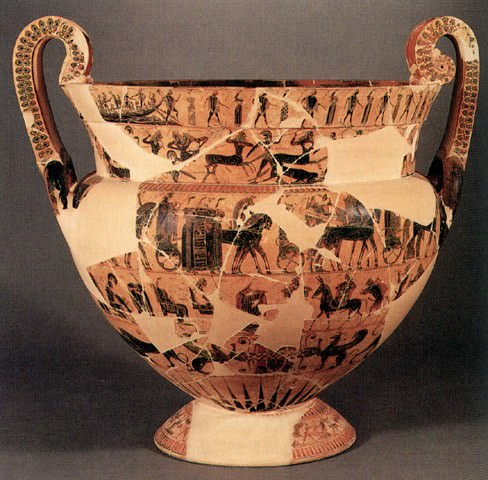
\includegraphics[height=0.25\textwidth]{pictures/terracotta_pot.jpg}
  \centering
\end{figure}


\subsection{Context}
This section will provide some basic knowledge
related to the jigsaw problem that will be useful
  for the next sections.
\subsubsection{Classification}
Puzzles are categorized in different types, for example:
\begin{itemize}
  \item Type 1 puzzles have the orientation of the pieces known, but the position unknown. 
  \item Type 2 puzzles have both the orientation and the position of the pieces unknown.
  \item Type 3 puzzles have the orientation of the pieces unknown, but the position known.
\end{itemize}
Between these categories type 2 are the hardest, and will be the focus of this paper.

\subsubsection{Digital vs Real-World Jigsaw Puzzles}

There is  another important distinction between different types of puzzles.
They can be divided into “digital” e.g.~\cref{fig:figure_digital_puzzle} and
“real world” e.g.~\cref{fig:figure_real_puzzle} jigsaw puzzles.
The difference between the two is quite self explanatory,
and can be observed in the respective pictures.
\label{document:DigitalVSReal}

% figure of digital jigsaw puzzle    
\begin{figure}[H]
    \caption{An example of a “digital” jigsaw  puzzle}\label{fig:figure_digital_puzzle}
    \centering
    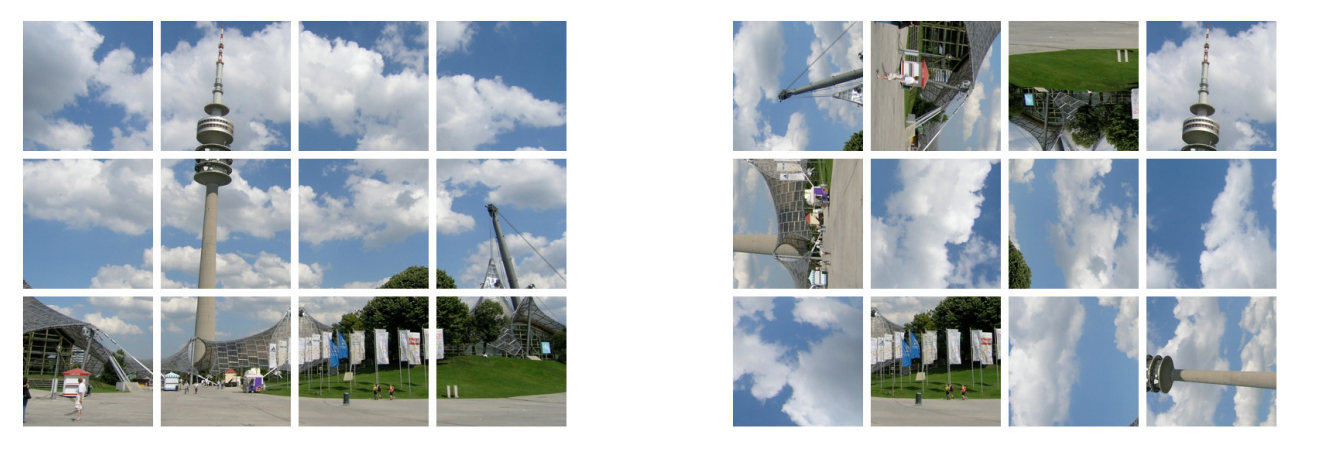
\includegraphics[height=0.25\textwidth]{pictures/digital_puzzle.png}
\end{figure}

% figure of real jigsaw puzzle    
\begin{figure}[H]
    \caption{An example of a ``real world'' jigsaw  puzzle}~\label{fig:figure_real_puzzle}
    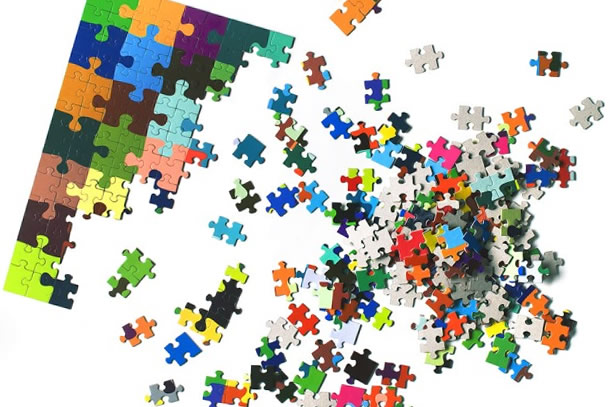
\includegraphics[height=0.25\textwidth]{pictures/real_puzzle.jpg}
    \centering

\end{figure}

The reason this distinction is important is because,
despite the generic concept of the puzzle not changing,
obtaining accurate measures of a piece's characteristics
is far easier with a digital puzzle,
since there are far fewer things that can go wrong.
For example, a piece's shape may be distorted by
a low-quality cut, as seen in~\cref{fig:figure_measurement_error}

% figure of a measurement error
\begin{figure}[H]
    \caption{An example of what can go wrong when dealing with the real world}\label{fig:figure_measurement_error}
    
\includegraphics[height=0.25\textwidth]{pictures/example_bad_piece.jpg}
    \centering
\end{figure}

\subsection{General Structure Of The Algorithms}

A puzzle solver program can be divided into 3 sub algorithms,
The Splitter, The Comparator and The Solver.
This generalization can be applied not only to our solution,
but also to all the algorithms analyzed in the related
work section of this paper (\cref{document:related_work}).

\begin{indented_section}

    \subsubsection{The Splitter:} This component takes as input one or more images
    containing all the pieces. It then separates all the pieces from each other,
    and split each piece into his four sides.\label{document:splitter}

    \subsubsection{The Comparator:} This component compares each side with all the
    others, in order to understand whether they match or not.\newline
    There are two distinct kinds of “Comparator” algorithms:
    The “Binary Comparison” and the “Non Binary Comparison”.
    As the name suggests when comparing two sides with a “Binary Comparison”
    the result can either be 0 (they do not match) or 1 (they match).
    In contrast a “Non Binary Comparison” can give any value between 0 and 1.
    This allows states of uncertainty to be represented.\label{document:comparator}

    \subsubsection{The Solver:} This component utilizes the information provided by the
    Comparator, and attempts to find a solution
    (i.e.\ a position and an orientation for each piece)
    that is the most likely to be correct.\label{document:solver}

\end{indented_section}


\subsection{The Objective Of This Paper}\label{document:objective}

This paper is not the first to tackle the jigsaw puzzle problem in computer science,
in fact there have been several more that are mentioned in the related work section (\cref{document:related_work}).

All the papers we read focused on digital jigsaw puzzles exclusively,
and we couldn't find any paper that mentioned real-world puzzles.
It should be mentioned that we did find some open source project that solved the
real-world puzzle problem, but they didn’t document the creation process nor the
findings given that they weren't trying to write a paper.

This paper’s objective is to focus on both digital and real-world jigsaw puzzles,
and document why the real-world version is harder, and try to quantify by how much.
In other to achieve this objective we want to answer these two questions:
\begin{itemize}
  \item \textbf{What is the difference in execution time between
                digital and real-world puzzles?}
  
  To answer this question we decided to build a puzzle solver from the ground up,
  and measure his performance across a set of digital, and real-world puzzles.
  Our focus when developing this component wasn't to build a state of the art algorithm,
  as there has already been extensive research put into that;
  We simply needed something that could work with both digital and real-world puzzles.
  
  \item \textbf{What are the challenges to use the current state of the art algorithms developed for digital
                puzzles in the real-world, and how can we overcome them?}
  
	Answering this question is a bit trickier, as an algorithm is divided into Comparator~\cref{document:comparator}
  and Solver~\cref{document:solver}. Due to the intrinsic difference of digital and real-world jigsaw puzzles
  reusing the Comparator is impossible, but there is the possibility to reuse the Solver,
  assuming we could build a Comparator for real-world puzzles that is in the same realm
  of accuracy achieved by Comparators for digital puzzles.
  So another way to write this question is: ``Can we build a Comparator for real-world
  puzzles that is accurate enough to work with current state-of-the-art  digital
  puzzle Solvers?''

	To answer this question we will measure the accuracy of the comparator we developed
  and observe what would happen if that accuracy is
  applied to a digital puzzle Solver. We will then propose a solution to improve
  the accuracy of real-world Comparators.


\end{itemize}

\subsection{The Dataset}
The last step of the introduction is defining our
testing dataset. We need both digital and real world
puzzles to solve. The dataset used, as well as
the code, can be seen in the public GitHub
repository:~\url{https://github.com/lucaSartore/PuzzleSolver}.
\label{document:dataset}
\subsubsection{The Real-World Puzzle}
The first step involves selecting a real-world
puzzle to solve. It has been decided to utilize a
classic 1000-piece puzzle measuring 66cm x 50cm.
A printer's scanner is employed to digitize the individual pieces.

The puzzle has been scanned in various sub-sizes to facilitate the testing of different configurations.
A resolution of 1200 pixels per inch (ppi) has been employed to ensure a sharp and precise
depiction of the pieces, as seen in~\cref{fig:figure_measurement_error}.
The puzzle has been scanned backward, using a black background.

This choice has been dictated by the fact that the scanner used has the flashlight
slightly off-centered from the scanner's sensor.
And this causes a shadows to be cast on one side of the pieces.
A black background has been chosen to solve the problem of the shadow.
And then the pieces has been flipped backward, since many of them where black,
and it was difficult to separate them from the background.
In the future it would be possible to scan the pieces in the correct orientation,
by using a different scanner.

\subsubsection{The Digital Puzzle}
The digital puzzles have been obtained from \url{https://puzzle.telegnom.org/}.
This web app can generate a puzzle from a dimension and a jitter value. The jitter is a parameter that controls
how unique and distorted the puzzle images are, see \cref{fig:jiiter}.
The default jitter used in the tests is 5\%.

\section{Our Implementation Of A Puzzle Solver}

This section will describe the implementation of the puzzle solver we developed.
This solver will then be put to the test in the next sections.

\subsection{Our Splitter}

\subsubsection{Splitting The Pieces}

As introduced in~\cref{document:splitter},  the initial stage in puzzle solving involves
splitting an image composed of many pieces into individual ones.
This is relatively straightforward, and can be done with the following steps:

\begin{itemize}
  \item Apply a threshold and transform an RGB image into a binary mask.
  \item Find all individual Blobs
  (a Blob is defined as a set of connected pixels with the same color) and for each one:

  \begin{itemize}
  \item Calculate the area (the number of pixels the Blob is made of)

  \item Add it to the set of pieces only if his area in within a certain range (to avoid small pieces of dust ending up counted as pieces)

  \end{itemize}

\end{itemize}

\subsubsection{Splitting The Sides}

The next step following the general structure described in~\cref{document:splitter}
is to split a piece into
his 4 sides, this can be done with the following steps:

\begin{itemize}

  \item \textbf{Remove the holes from the piece:}\newline
  To remove the holes from the piece, the program employs a three-step process. Initially it
  computes the convex hull of the piece~\cref{fig:s_s_ch}.
  Subsequently it calculates the difference between the convex hull and the original image,
  resulting in an ``image with filler areas''~\cref{fig:fig:s_s_og_minus_ch}.
  It can be noted that these filler areas have distinct shapes,
  depending on what has generated them (either a ``hole'' or a ``knob'').
  Therefore they can be categorized.
  Finally the filler areas are added back to the original only if
  they originated from a hole. This results in an image where the holes
  have been filled~\cref{fig:s_s_no_holes}

  \item \textbf{Remove the knobs from he piece:}\newline
  In order to remove the knobs from the piece, the image without holes
  undergoes an erosion~\cref{fig:s_s_erosion} followed by a dilation~\cref{fig:s_s_dilatation}.
  This process results in an image that resembles the original, but without any knobs.
  Subsequently, the program identifies the pixels that are white in the image without holes~\cref{fig:s_s_no_holes},
  but not in the eroded and dilated version~\cref{fig:s_s_dilatation}.
  This leads to the formation of a set of blobs ~\cref{fig:s_s_no_holes_minus_expansion}.
  It is important to note that the shape of a blob can vary significantly depending on whether it originated
  from an ``angle'' or a ``knob'' and thus they can be classified accordingly.
  Following this, the program proceeds to eliminate from the hole-free
  image~\cref{fig:s_s_no_holes} all pixels that are in close proximity to a blob generated by a knob.
  This operation yields an image that is both devoid of knobs and holes~\cref{fig:s_s_no_knobs}.
  
  \item \textbf{Find the coordinates of the four corners:}\newline
  In order to determine the coordinates of the corners,
  the program employs a three-step approximation method.
  Initially, it identifies the minimum enclosing rectangle and
  utilizes the coordinates of its corners
  as the first approximation~\cref{fig:s_s_min_enc_rec}.\newline
  For the second approximation, the program selects,
  from the white pixels in close proximity to the first approximation,
  the pixel that contains the highest number of black pixels
  within a specified range.
  Then it considers only the pixels that are within a certain
  distance of the second approximation, and finds the minimum
  enclosing triangle of sed pixels~\cref{fig:s_s_min_enc_triangle}.\newline
  The corner of the triangle that is nearest to the second
  approximation serves as the third and final approximation
  for the corner of the puzzle piece.
  The position of the four corners can be seen in image~\cref{fig:s_s_corners_found}.

  \item \textbf{Split each piece into four sides using the previously found coordinates:}\newline
	After the program has successfully identified the four corner coordinates,
  it can straightforwardly derive each of the four sides.
  An example of a single side can be seen in image .~\cref{fig:s_s_a_piece_side}.
\end{itemize}

\begin{figure}
  \begin{subfigure}{0.3\textwidth}
    \centering
    
\includegraphics[width=\linewidth]{pictures/original_piece.jpeg}
    \caption{Original binary mask of a piece.}
    \label{fig:s_s_og}
  \end{subfigure}
  \hfill
  \begin{subfigure}{0.3\textwidth}
    \centering
    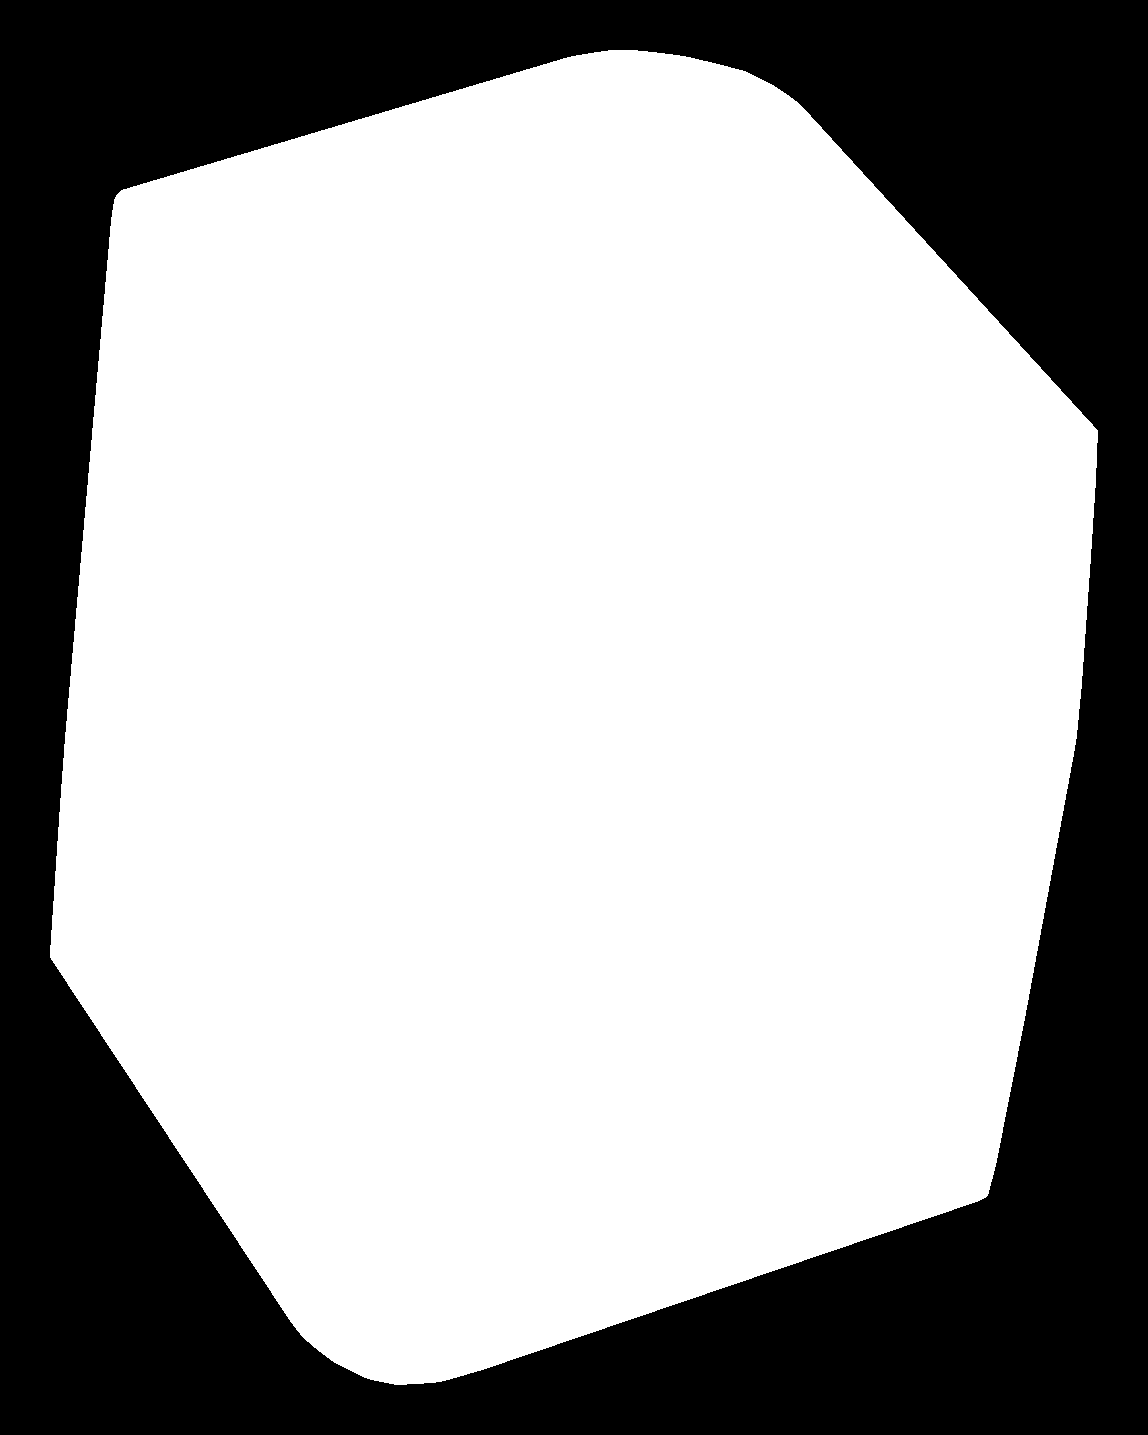
\includegraphics[width=\linewidth]{pictures/remove_holes_convex_hull.png}
    \caption{Convex Hull of a piece.}
    \label{fig:s_s_ch}
  \end{subfigure}
  \hfill
  \begin{subfigure}{0.3\textwidth}
    \centering
    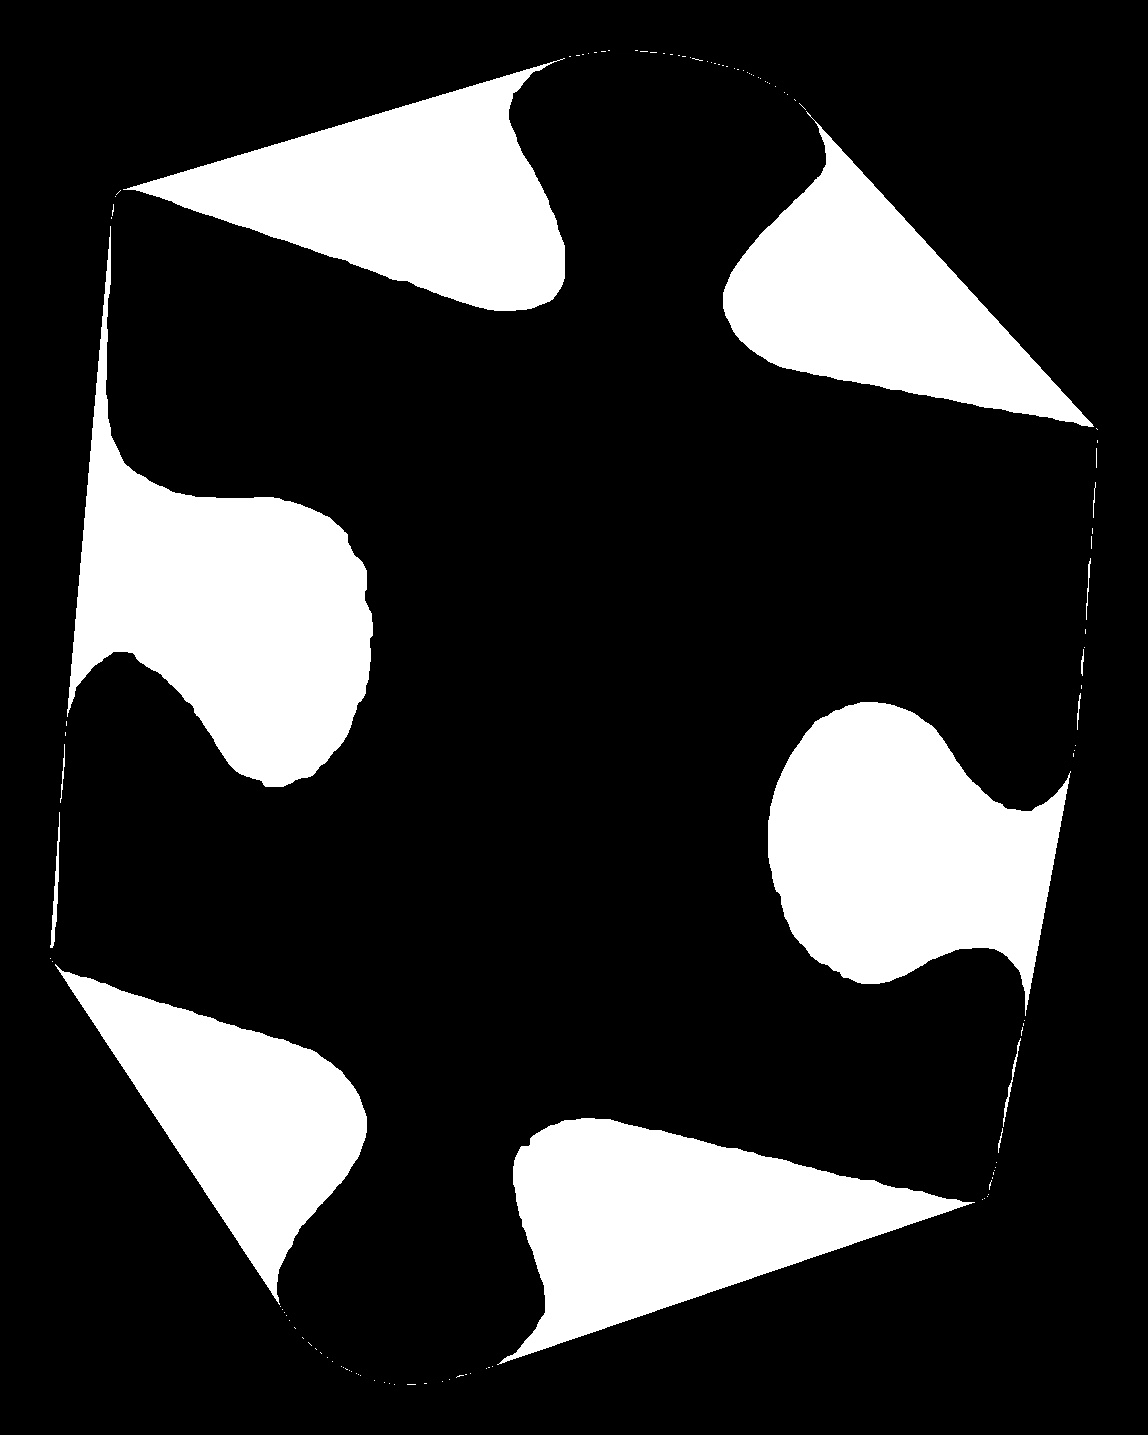
\includegraphics[width=\linewidth]{pictures/remove_holes_filler_areas.png}
    \caption{Difference:~\cref{fig:s_s_ch} \textminus~\cref{fig:s_s_og}.}
    \label{fig:fig:s_s_og_minus_ch}
  \end{subfigure}
  \vspace{1cm}
  \begin{subfigure}{0.3\textwidth}
    \centering
    
\includegraphics[width=\linewidth]{pictures/piece_with_no_hole.png}
    \caption{Piece~\cref{fig:s_s_og} with holes removed.}
    \label{fig:s_s_no_holes}
  \end{subfigure}
  \hfill
  \begin{subfigure}{0.3\textwidth}
    \centering
    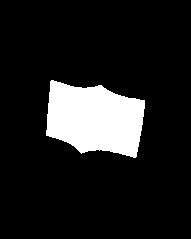
\includegraphics[width=\linewidth]{pictures/remove_knobs_erosion.png}
    \caption{Mask~\cref{fig:s_s_no_holes} eroded.}
    \label{fig:s_s_erosion}
  \end{subfigure}
  \hfill
  \begin{subfigure}{0.3\textwidth}
    \centering
    
\includegraphics[width=\linewidth]{pictures/remove_knobs_expansion.png}
    \caption{Mask~\cref{fig:s_s_erosion} dilated.}
    \label{fig:s_s_dilatation}
  \end{subfigure}
  \vspace{1cm}
  \begin{subfigure}{0.3\textwidth}
    \centering
    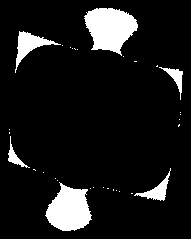
\includegraphics[width=\linewidth]{pictures/remove_knobs_knob_pixels.png}
    \caption{Difference:~\cref{fig:s_s_no_holes} \textminus~\cref{fig:s_s_dilatation}.}
    \label{fig:s_s_no_holes_minus_expansion}
  \end{subfigure}
  \hfill
  \begin{subfigure}{0.3\textwidth}
    \centering
    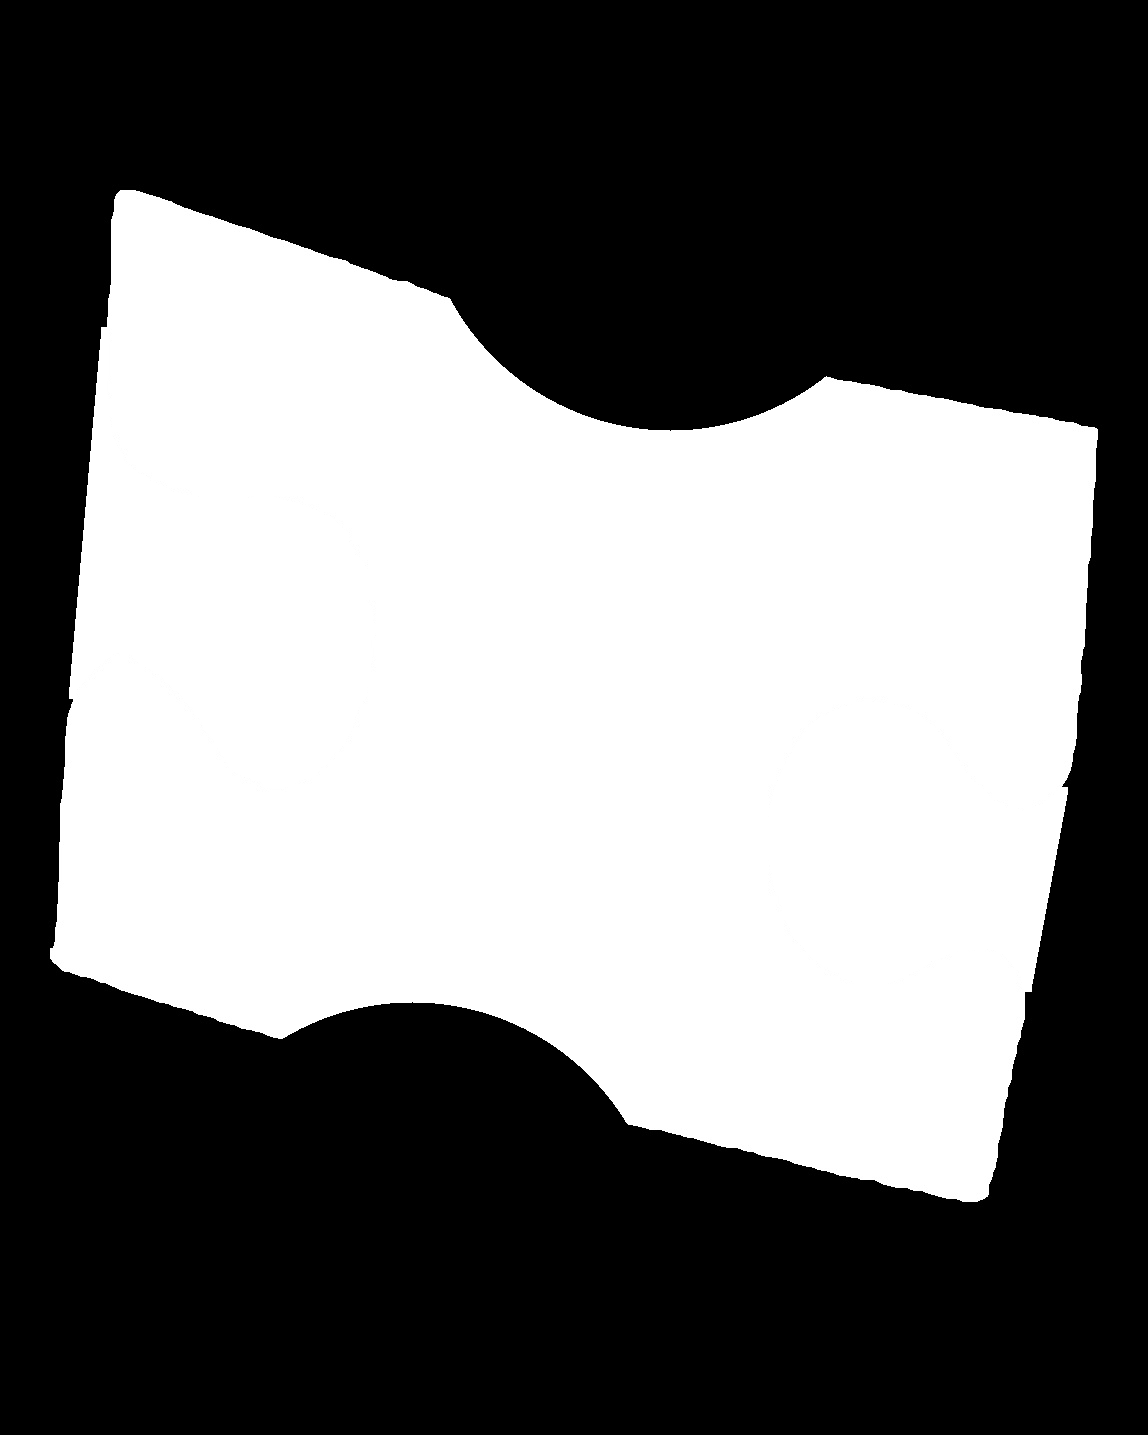
\includegraphics[width=\linewidth]{pictures/piece_with_no_knobs.png}
    \caption{Piece~\cref{fig:s_s_no_holes} with knobs removed.}
    \label{fig:s_s_no_knobs}
  \end{subfigure}
  \hfill
  \begin{subfigure}{0.3\textwidth}
    \centering
    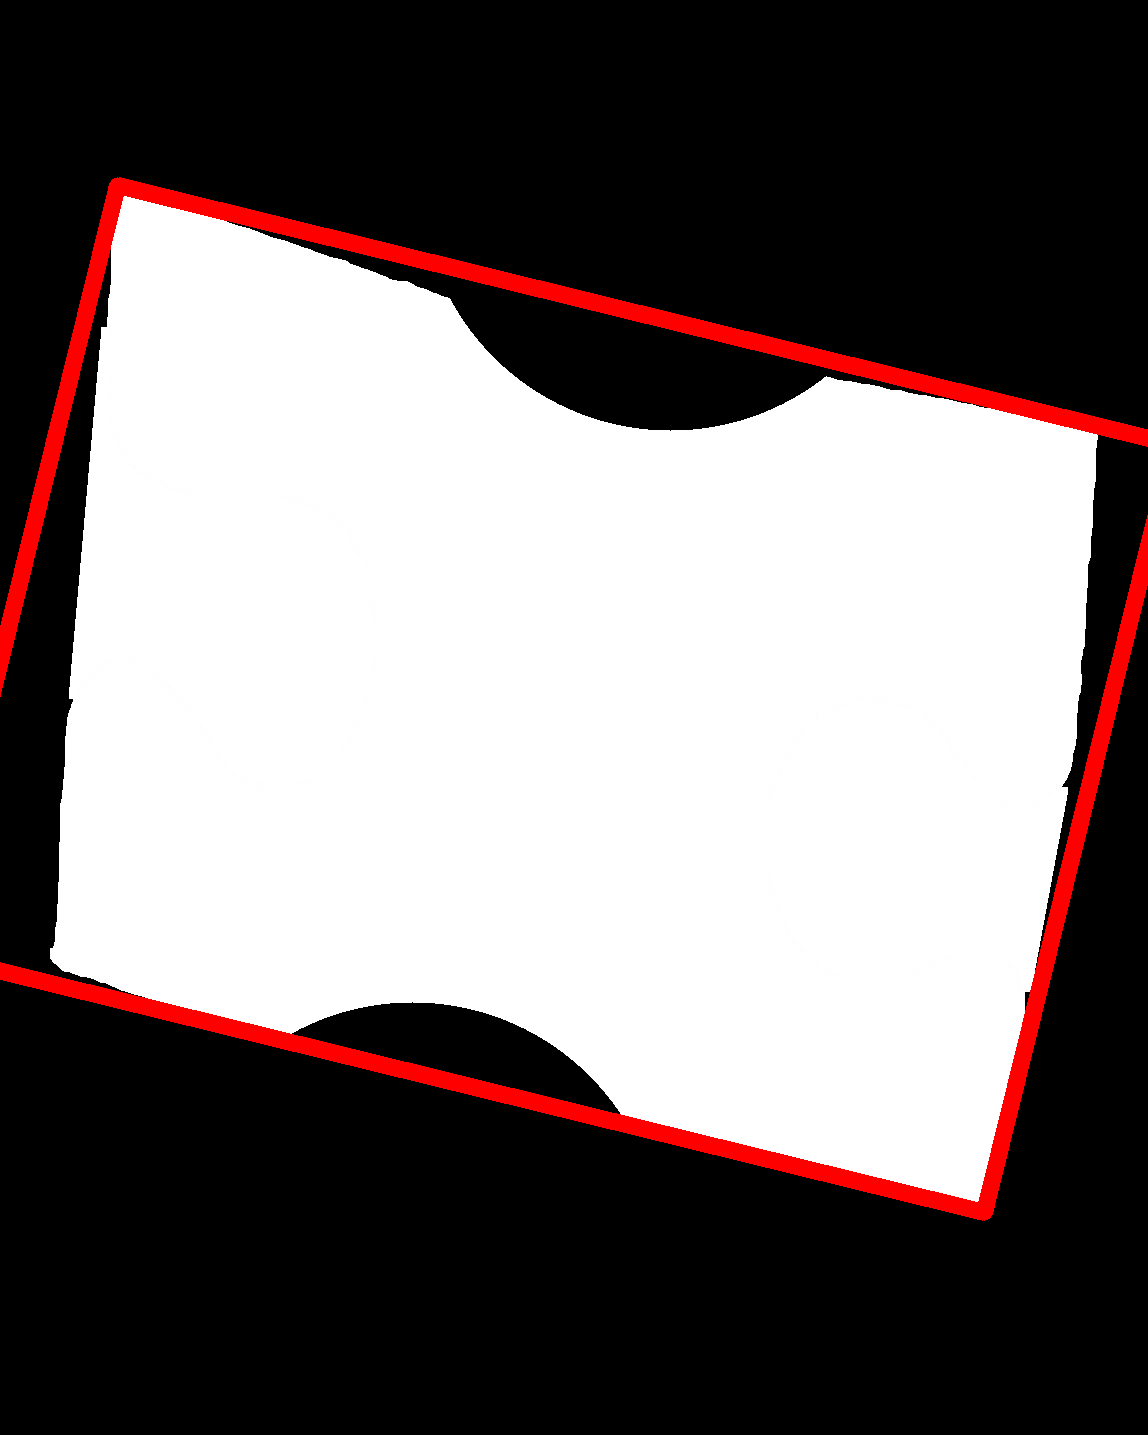
\includegraphics[width=\linewidth]{pictures/find_corners_min_enclosing_rectangle.png}
    \caption{Min enclosing rectangle of~\cref{fig:s_s_no_knobs}.}
    \label{fig:s_s_min_enc_rec}
  \end{subfigure}
\end{figure}
\clearpage
\begin{figure}\ContinuedFloat
  \begin{subfigure}{0.3\textwidth}
    \centering
    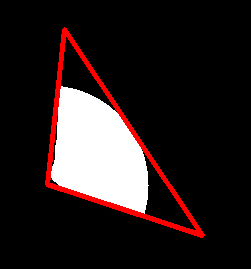
\includegraphics[width=\linewidth]{pictures/find_corners_min_enclosing_triangle.png}
    \caption{Min enclosing triangle of the bottom right corner of~\cref{fig:s_s_no_knobs}.}
    \label{fig:s_s_min_enc_triangle}
  \end{subfigure}
  \hfill
  \begin{subfigure}{0.3\textwidth}
    \centering
    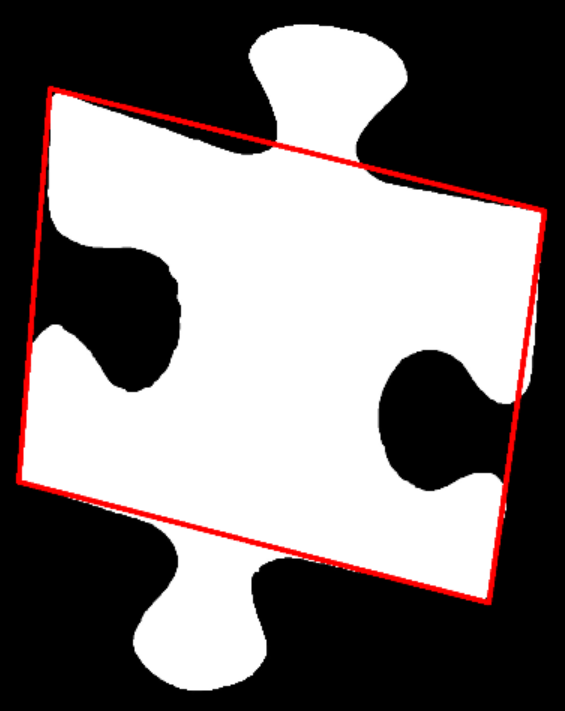
\includegraphics[width=\linewidth]{pictures/corners_found.png}
    \caption{The corners of the piece~\cref{fig:s_s_og}.}
    \label{fig:s_s_corners_found}
  \end{subfigure}
  \hfill
  \begin{subfigure}{0.3\textwidth}
    \centering
    
\includegraphics[width=\linewidth]{pictures/piece_side.png}
    \caption{One of the sides of the piece~\cref{fig:s_s_og}.}
    \label{fig:s_s_a_piece_side}
  \end{subfigure}
  
  \caption{Steps needed to split an image into his four sides.}
  \label{fig:splitting_sides}
  
\end{figure}



\subsection{Our Comparator}\label{document:my_comparator}
The next step is to compare the sides that have been
generated before, in order to generate
a compatibility shore.
To achieve this, the program employs
the following steps:

\begin{itemize}
  \item For each side, it considers only the border, and  makes it thicker.
  \item It puts two sides attached to each other using the coordinates of the corners (In the same way a human would do to test if two pieces fit together).
  \item It calculates the “Or Area”; that is, the number of pixels that belong to the border of one side or the other.
  \item It calculates the “And Area”; that is, the number of pixels that belong to the border of both sides.
  \item It calculates the final shore, which is defined as: \(Shore = \frac{And \space Area}{Or \space Area}\), and goes from 0 to 1.
\end{itemize}


\begin{figure}[htbp]
  \centering
  \begin{minipage}[t]{0.44\textwidth}
    \vspace{3pt} % Ensure alignment of the top of the minipage
    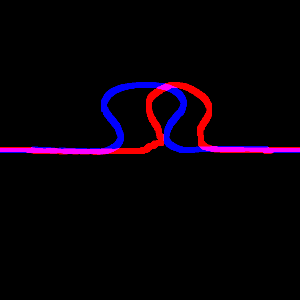
\includegraphics[width=\textwidth]{pictures/side_comparation.png}
  \end{minipage}
  \hfill
  \begin{minipage}[t]{0.54\textwidth}
    \caption{\newline
    In this image we can see two sides that have been
    compared, one side is drowned in red, the other one in blue.
    In this picture, the “Or Area” is represented by all non
    black pixels; The “And Area” is represented by all the
    purple pixels.}
  \end{minipage}
\end{figure}
\clearpage



\subsection{Our Solver}\label{document:my_solver}
The Solver we developed cannot be considered state-of-the-art when compared
to the current best digital puzzle solvers. However, it may be
considered as such when compared to existing ``real-world'' puzzle solvers.

Regardless, the achieved performances are still good enough to test and understand
the differences between digital and real-world puzzles,
which is the main objective of this paper.

\subsubsection{Overview}
The algorithm itself is relatively straightforward.
It operates as a recursive procedure, initiating by recognizing all 2x2
sets of matching pieces through the combination of four individual pieces.
Subsequently, it extends this process to identify all 4x4 sets of matching pieces
by aggregating four 2x2 pieces, and this pattern continues recursively.

\subsubsection{Basic Components}
To implement the algorithm two fundamental object are defined
\begin{itemize}
  \item \texttt{SinglePiece}: which contains information about a single puzzle piece.
  \item P\texttt{PieceGroup\(<\)T\(>\)} where \texttt{T} can be either a \texttt{PieceGroup} or a \texttt{SinglePiece}\newline
  This element encompasses four elements of type \texttt{T}, each with its own position (top right, top left, bottom left, bottom right).
\end{itemize}
Both \texttt{SinglePiece} and \texttt{PieceGroup} have an ``orientation'' attribute that goes from 0 to 3, this attribute
represent the orientation of the piece, as shown in~\cref{fig:orientation}.
\begin{figure}[H]
  \caption{orientation attribute of an object}\label{fig:orientation}
  \centering
  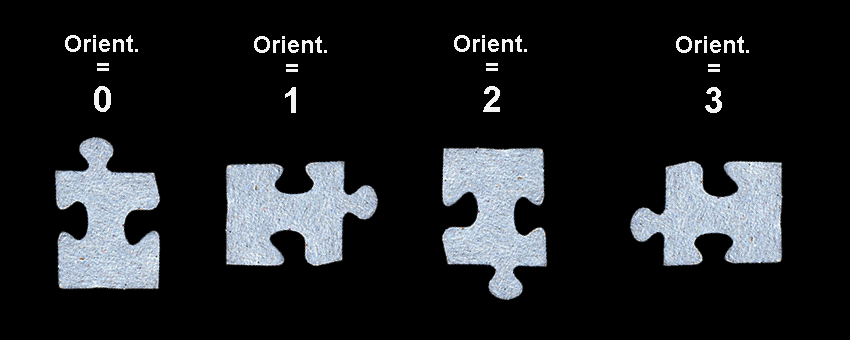
\includegraphics[height=0.3\textwidth]{pictures/orientation.png}
\end{figure}

\subsubsection{The Levels}

These objects are assigned levels:
\begin{itemize}
\item \texttt{SinglePiece} is at level 0, representing a 1x1 ``solution'' to a puzzle.
\item \texttt{PieceGroup\(<\)SinglePiece\(>\)} is at level 1, representing a 2x2 solution to a puzzle.
\item \texttt{PieceGroup\(<\)PieceGroup\(<\)SinglePiece\(>>\)} is at level 2, representing a 4x4 solution to a puzzle, and so forth.
\end{itemize}

\subsubsection{The Behaviors}

These basic objects also have the following shared behaviors:
\begin{itemize}
  \item 4 objects of level N can be combined to build an object of level N+1.
  \item One object of level N has 4 sides, each of which can be compared with a side of an element of level N. This results in a compatibility shore.
  \begin{itemize}
    \item The comparing shore for level 0 objects is just the shore given by the Comparator of~\cref{document:comparator}.
    \item The comparing shore for level N+1 objects is the average between two comparisons made with objects of level N
  \end{itemize}
\end{itemize}

\subsubsection{Combining four objects}\label{document:combining_four_objects}
When combining four objects into one, some comparisons are executed to
ensure that the resulting piece is a valid  combination.

\begin{itemize}
  \item The right side of the object in the top left position is compared with the left side of the object in the top right position~\cref{fig:merge_pieces}(1).
  \item The bottom side of the objection the top right position is compared with the top side of the object in the bottom right position~\cref{fig:merge_pieces}(2).
  \item The left side of the objection the bottom right position is compared with the right side of the object in the bottom left position~\cref{fig:merge_pieces}(3).
  \item The top side of the objection the bottom left position is compared with the bottom side of the object in the top left position~\cref{fig:merge_pieces}(4).
\end{itemize}

\begin{figure}[H]
  \caption{Example of a combination of four objects in to one}\label{fig:merge_pieces}
  \centering
  \includegraphics[height=0.3\textwidth]{pictures/merge_pieces.png}
\end{figure}

In order for the created object to be considered valid all of the comparisons must have a shore greater
than the constant \texttt{MIN\_SHORE\_SINGLE\_SIDE}. And the average of the four comparisons must be greater
than the constant \texttt{MIN\_SHORE\_PIECE\_GROUP}.

The process also checks that all individual pieces inside a newly
created object are different (because obviously is impossible to reuse the same piece twice to solve a puzzle)
\subsubsection{The Algorithm}

As mentioned earlier, the algorithm is implemented with a recursive function.
The function is generic, and can take as input objects of any level.

A Function of level N takes as input a list of objects of level N,
and creates all possible objects with level N+1.
Then it uses the newly created objects to generate a recursive call on a version
of itself with level N+1.
This process is repeated until the desired size is reached.


\begin{minipage}{\textwidth}
\begin{lstlisting}
  # This function returns a list of object that match with `piece_to_match'
  # along the direction `direction'.
  # It also filters the data to return only pieces with an index greater than `index_filter'
  # This function is executed in constant time, since it relies on some pre-processing of the data
  def get_matches(piece_to_match, direction, index_filter):
      ...

  def solve<T>(pieces: List<T>):

      number_of_pieces = pieces.length()

      found_pieces = List::<PieceGroup<T>>::new()

      # this function compare all pieces with the others, and build some data structures
      # that are used from the function `get_matches'
	   # the time complexity is o(N^2)
      do_pre_processing(pieces)

      # test all possible combinations for the top left piece
      for top_left_index in 0..number_of_pieces:
	       for top_left_orientation in 0..4:

          # get the top left piece
          top_left = get_piece(top_left_index, top_left_orientation)

          # test all possible combinations of top_right, bottom_right and bottom_left
          for top_right in get_matches(top_left, RIGHT, top_left_index):
	           for bottom_right in get_matches(top_right, DOWN , top_left_index):
                  for bottom_left in get_matches(bottom_right, LEFT, top_left_index):

                      # try to create the new piece group
                      new_element = PieceGroup::new(top_left, top_right, bottom_right,bottom_left)

                      if new_element.is_valid():
                          # if the 4 pieces can fit together the newly created piece
                          # is added to the list of found pieces
                          found_pieces.add_element(new_element)
                      else:
                          # otherwise the program check what the case of the 
                          # invalid creation is, and generate a continue
                          # on the respective loop, to speed up the operations
                          continue_failure_cause_loop()

      # at the end a recursive call is generated 
      return solve::<PieceGroup<T>>(found_pieces)

\end{lstlisting}
\end{minipage}
The procedure begins by testing all possible pieces and orientations as the top\_right piece.
Then continues by finding all the other 3 pieces in an efficient way thanks to get\_matches.
When the program has an hypothesis on the 4 pieces that can build a new piece it tries to create it.\newline
The creation process does some checks, and if everything is successful it adds the piece to the list of found pieces.
If the creation is not successful it figures out which piece has caused the failure, and moves to the next iteration of the respective loop.\newline
When all combinations have been found, the function makes a recursive call and the process is repeated.\newline
The process ensures that the piece in the top\_left is always the one with the lower index.
This is done to avoid building the same piece 4 times with 4 different orientations.\newline
One advantage of this algorithm is that the outer edge for loop can be easily parallelized to achieve better performances.


It should be noted that this pseudo code omits many details, two of witch are:
\begin{itemize}
  \item A condition that checks if the desired size has been reached and eventually stops the recursion.
  \item A condition that specifically handles cases where the final size of the puzzle can't be reached simply by combining 4 pieces together recursively.
  Without this condition the algorithm could only solve squared puzzles. Who's size is a power of 2. 
\end{itemize}

\section{Related work}\label{document:related_work}
Now that we have developed our own solution, it would be
interesting to see how it compares against the current
state-of-the-art algorithms for both digital and real-world
jigsaw puzzles. This section gives a brief introduction to 3
state-of-the-art algorithms, so that they can be compared with
our solution in the conclusions.

\subsection{Solving Jigsaw Puzzles By The Graph Connection Laplacian~\cite{GCL}}
This algorithm falls within the ``binary comparison'' category (\cref{document:comparator}).
And can be used to understand the strength and weaknesses
of this approach.\newline
The primary advantage of this approach lies in its speed;
the utilization of binary comparison permits specific optimizations,
particularly leveraging graph theory techniques.\newline
The algorithm exhibits a time complexity of approximately \(O(N^2)\),
a value consistent with the theoretical minimum for
jigsaw puzzle solving, as outlined in the study
``No easy puzzles: Hardness results for jigsaw puzzles~\cite{ON2Claim}''.\newline
However, a potential drawback may arise in terms of accuracy.
This stems from the fact that, with only two states
(matching or not matching),
certain details may be lost when compared to a non-binary comparison. 
To quantify accuracy the paper used the ``neighbors comparison'' metric,
which ``calculates the percentage of pairs of image patches that are matched correctly''.
This will be useful later.\label{document:GCL}

\subsection{A Genetic Algorithm-Based Solver for Very Large Jigsaw Puzzles~\cite{GA}}
This paper employs genetic algorithms to address the
jigsaw puzzle problem, yielding promising results.\newline
The algorithm seems to have a \(O(N^2)\) time complexity,
with execution time slightly lower than the previous example
(However, it remains uncertain which one is faster, as the papers did not specify
the particular hardware configuration used).\newline
The paper adopts the same evaluation method for accuracy as the previous example,
namely neighbor comparison, facilitating direct comparison between the two approaches.
This algorithm falls under the category of “Non binary comparison”~\cref{document:comparator}
a distinction that theoretically grants it an advantage due to the increased granularity
of input data.
Unfortunately this advantage does not compensate for the worst precision
of the algorithm itself, and the accuracy results are equivalent,
if not slightly worse than the previous algorithm.\newline
It is important to keep in mind that for the very nature of genetic algorithms,
it might be possible that the accuracy would have been better if they had allowed
the algorithm to run for more generations.\label{document:GA}

\subsection{Computer Vision Powers Automatic Jigsaw Puzzle Solver~\cite{Abto}}
Solutions~\cref{document:GCL} and~\cref{document:GA} can be considered ``state-of-the-art''
for digital jigsaw puzzles.
However, as already introduced in section ~\cref{document:DigitalVSReal},
translating these solutions to the real world can be challenging.\newline
This article represents one of the most comprehensive and well-documented
implementations for real-world puzzles. However,
it's important to note that referring to this approach as a ``solution''
may be misleading, as it primarily identifies the top eight matching
pieces for a specific point and subsequently relies on user input to make
the final placement decision.
This aspect renders the algorithm non-autonomous..\newline
Even disregarding this significant detail,
conducting an analysis of this solution has proven to be challenging,
as the article leans more towards a publicity stunt than an academic paper.
In fact, the code is not open source, and informations regarding the time needed
to solve the puzzle are absent. The article only showcases a single puzzle solved,
with dimensions of 9\(\times\)6.\newline
Despite these limitations, this article still stands as one of the best examples of a solution
for real-world puzzles.



\section{Evaluation}
This section will evaluate the proposed solution by measuring
two key metrics: execution time and accuracy. 
The objective of this section is to answer the first question posed in~\cref{document:objective}:
\begin{itemize}
  \item What is the difference in execution time between
                digital and real-world puzzles?
\end{itemize}

\subsection{Execution Time Analysis}

This section measures the execution time of many puzzles,
and shows the results. The puzzles that has been used for
this test has been described in ~\cref{document:dataset}.

The constants \texttt{MIN\_SHORE\_SINGLE\_SIDE} and \texttt{MIN\_SHORE\_PIECE\_GROUP} mentioned in
section~\cref{document:combining_four_objects} were set at different values
depending on the nature of the puzzle (real or digital).

The test has been performed on a ryzen 5 5600 CPU with 16 GB of RAM.
The time measured in the test does not include the execution time of the Comparator
\cref{document:my_comparator}, but only the one of the Solver~\cref{document:my_solver}.

\subsubsection{Digital vs Real World Puzzles}

In the table below we can see how the same algorithm
can have vastly different performance depending on the kind of puzzle 
it is working with.
\begin{table}[H]
  \centering
  \begin{tabular}{
  >{\columncolor[HTML]{D9EAD3}}c 
  >{\columncolor[HTML]{D0E0E3}}c 
  >{\columncolor[HTML]{F4CCCC}}c 
  >{\columncolor[HTML]{FCE5CD}}c }
  \cellcolor[HTML]{B6D7A8} &
    \cellcolor[HTML]{A2C4C9} &
    \multicolumn{2}{c}{\cellcolor[HTML]{EA9999}Execution time {[}s{]}} \\
  \multirow{-2}{*}{\cellcolor[HTML]{B6D7A8}Size} &
    \multirow{-2}{*}{\cellcolor[HTML]{A2C4C9}Pieces} &
    \cellcolor[HTML]{DD7E6B}Digital puzzle &
    \cellcolor[HTML]{F9CB9C}Real Puzzle \\
  2x3   & 6   & 1   & 4    \\
  3x4   & 12  & 3   & 14   \\
  4x4   & 16  & 4   & 59   \\
  4x5   & 20  & 4   & 48   \\
  5x8   & 40  & 20  & 627  \\
  8x8   & 64  & 30  & 2851 \\
  8x12  & 96  & 660 & N/A  \\
  16x16 & 256 & 377 & N/A 
  \end{tabular}
\end{table}

Looking at the data we can spot to anomalies:
\begin{itemize}
  \item The 4x5 real puzzle has a lower execution time than the 4x4 real puzzle. This is not a big
  difference and can be attribute to run to run variation.
  \item The 8x12 digital puzzle has a much higher execution time than the 16x16 digital puzzle.
  This is also easily explainable, as puzzles whose side is not a power of two are in general
  harder compared to those who fulfill this condition. As they require an extra step compared to
  the simple algorithm shown in~\cref{document:my_solver}.
\end{itemize}

\subsubsection{Effect of Jitter on Execution Time}

As mention in \cref{document:dataset} the digital puzzle have an attribute called jitter.
Intuitively increasing the jitter would make the pieces harder to
match with each other, and consequently making the puzzle easier to solve.
And we can observe that this intuition is correct in the table below.

\begin{figure}[h]
  \caption{Effect of jitter on jigsaw pieces}\label{fig:jiiter}
  \centering
  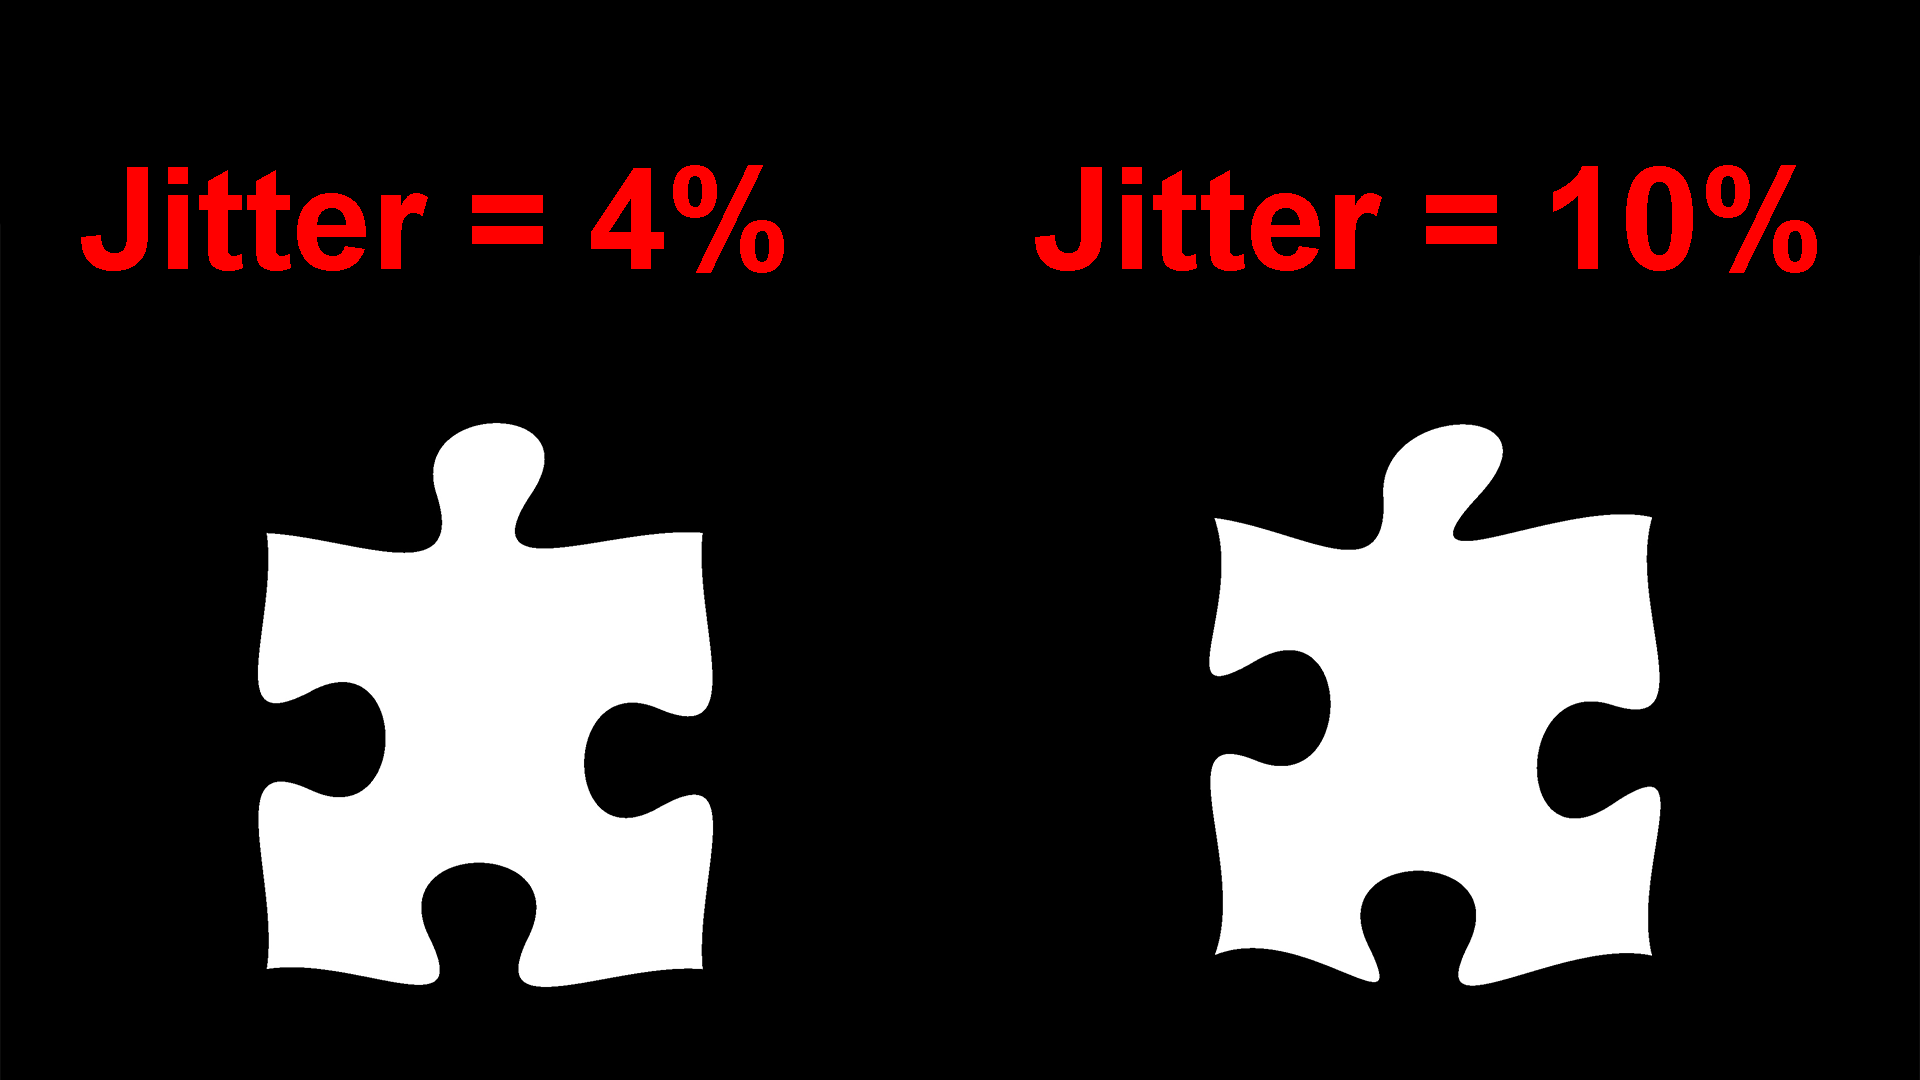
\includegraphics[height=0.3\textwidth]{pictures/jitter.png}
\end{figure}

\begin{table}[H]
  \centering
  \begin{tabular}{
  >{\columncolor[HTML]{D0E0E3}}c 
  >{\columncolor[HTML]{C9DAF8}}c }
  \multicolumn{2}{c}{\cellcolor[HTML]{B6D7A8}Jitter effect on an 8x8 digital puzzle} \\
  \cellcolor[HTML]{A2C4C9}Jitter   & \cellcolor[HTML]{A4C2F4}Execution time {[}s{]}  \\
  4\%                              & 104                                             \\
  5\%                              & 30                                              \\
  6\%                              & 17                                              \\
  8\%                              & 17                                              \\
  10\%                             & 16                                             
  \end{tabular}
  \end{table}

This shows how the execution time can be six times faster just by making
each piece more unique.
\subsubsection{Run to Run Variation}

Another feature of the algorithm that is worth testing is his consistency.
To measure tested the performance on 5 distinct puzzles, with the only thing in common
been a size of 4$\times$4.

\begin{table}[H]
  \centering
  \begin{tabular}{
  >{\columncolor[HTML]{FCE5CD}}c 
  >{\columncolor[HTML]{FFF2CC}}c 
  >{\columncolor[HTML]{EAD1DC}}c }
  \multicolumn{3}{c}{\cellcolor[HTML]{EA9999}Run to run variance on a 4x4 real puzzle}                                                             \\
  \cellcolor[HTML]{F9CB9C}Execution time {[}s{]} & \cellcolor[HTML]{FFE599}Average                 & \cellcolor[HTML]{D5A6BD}Standard deviation     \\
  64 & \cellcolor[HTML]{FFF2CC} & \cellcolor[HTML]{EAD1DC} \\
  68 & \cellcolor[HTML]{FFF2CC} & \cellcolor[HTML]{EAD1DC} \\
  43 & \cellcolor[HTML]{FFF2CC} & \cellcolor[HTML]{EAD1DC} \\
  24 & \cellcolor[HTML]{FFF2CC} & \cellcolor[HTML]{EAD1DC} \\
  29 & \cellcolor[HTML]{FFF2CC} & \cellcolor[HTML]{EAD1DC} \\
  59 & \multirow{-6}{*}{\cellcolor[HTML]{FFF2CC}47.8} & \multirow{-6}{*}{\cellcolor[HTML]{EAD1DC}18.6}
\end{tabular}
\end{table}

\subsubsection{Accuracy}
It is crucial to mention that the project currently lacks an automated
method for evaluating the accuracy of the results. However, the accuracy
of two real-world puzzles (4x4 and 8x8) and one digital puzzle (16x16) has been manually confirmed,
with them achieving a 100\% correctness.

\begin{table}[H]
\centering
\begin{tabular}{
>{\columncolor[HTML]{FCE5CD}}c 
>{\columncolor[HTML]{FFF2CC}}c 
>{\columncolor[HTML]{EAD1DC}}c }
\multicolumn{3}{c}{\cellcolor[HTML]{EA9999}Manually evaluated accuracy of the solutions}                       \\
\cellcolor[HTML]{F9CB9C}Puzzle size & \cellcolor[HTML]{FFE599}Puzzle kind & \cellcolor[HTML]{D5A6BD}Accuracy \\
4x4                                 & real world                          & 100\%                            \\
8x8                                 & real world                          & 100\%                            \\
16x16                               & digital                             & 100\%                           
\end{tabular}
\end{table}

\subsubsection{Answering The Question}

This paper has asserted from the beginning that real-world puzzles
pose greater challenges compared to their digital counterparts.
While some intuitive explanations were provided to support this assertion,
a proof hasn't been presented until now. This test ultimately substantiates 
the claim, demonstrating that the performance of the same
algorithm can vary significantly depending on the accuracy of the input data.

\section{Conclusion}

This sections aim to conclude the paper by answering the second question
posed in ~\cref{document:objective}:

\begin{itemize}
  \item What are the challenges to use the current state of the art algorithms developed for digital
                puzzles in the real-world, and how can we overcome them?
\end{itemize} 

Ath the end of the section we will also make some consideration about
possible future works related to this problem.

\subsection{Applying Already Existing Algorithms To The Real World}

Comparing the results achieved by our algorithm with some of the algorithms seen in the related
work section (\cref{document:related_work}), clearly shows how our algorithm is far away
from the current state-of-the-art digital puzzle solvers. In this section we want to
see if it is possible to use our comparator with current state-of-the-art algorithms.
In particular we selected the ``Graph Connection Laplacian''~\cite{GCL} solution, due to the
comprehensive details provided in the paper. Notably, it contains information
regarding the algorithm's accuracy in relation to the corruption rate,
which is crucial for this analysis.

Unfortunately the conducted tests reveal that the Comparator we developed in~\cref{document:my_comparator}
and the ``Graph Connection Laplacian'' solution of~\cref{document:GCL}
are not compatible with each other.
A proof supporting this assertion is presented subsequently.


\subsubsection{Selecting The Threshold Based On Input Data}

The comparison algorithm described in~\cref{document:my_comparator} outputs a compatibility
shore that goes from 0 to 1.\newline
But the graph connection Laplacian algorithm of~\cref{document:GCL} takes as input a binary value.
Which means that it is necessary to apply a threshold to the input
data to convert them from float to bool.

To find the optimal threshold we solved a small 16 piece puzzle.
And we measured the following 4 values in function of the threshold:

\begin{itemize}
  \item \textbf{match\%:}\newline
  The probability that 2 randomly selected sides matches.
  
  \item \textbf{correct combination match\% (or c.c match\%):}\newline
  The probability that 2 randomly selected sides matches given that in the correct puzzle
  solution they are actually close to each other. Ideally this should be 1, as we would prefer
  that the comparison never returns false if two pieces are actually connected in the correct solution.
  
  \item \textbf{limit match\%:}\newline
  Given that this measures has been taken on a 16 piece puzzle,
  the match\% is highly influenced by the correct piece matching together.
  With a bigger puzzle the match\% would be lower (Given that the amount
  of correct couple of sides scales with N, while the amount of
  possible couple of sides scales with \(N^2\). Where N is the number of pieces).\newline
  Limit match\% is an approximation of what the match\%
  would be in the limit for \(N \rightarrow + \infty\).
  This value is obtained by subtracting to match\%
  the probability of choosing randomly the correct side,
  multiplied by the probability that the comparison returns true
  (which is c.c match\%).\newline
  Ideally limit match\% should be almost zero, as we would prefer that the comparison is true only when
  the pieces are actually connected in the correct solution.
  \[limit \: math\% = math\% - \frac{c.c. \: mathc\%}{16 \times 4}\]
  
  \item \textbf{corruption rate:}\newline
  Is defined as: \(1-\sqrt{c.c \: match\%}\). Ideally this should be 0.

\end{itemize}


\begin{table}[H]
  \centering
  \begin{tabular}{
  >{\columncolor[HTML]{FFE599}}c 
  >{\columncolor[HTML]{B6D7A8}}c 
  >{\columncolor[HTML]{9FC5E8}}c 
  >{\columncolor[HTML]{F9CB9C}}c 
  >{\columncolor[HTML]{D9D2E9}}c }
  \cline{1-1}
  \multicolumn{1}{|c|}{\cellcolor[HTML]{F1C232}threshold} &
    \cellcolor[HTML]{6AA84F}match\% &
    \cellcolor[HTML]{3C78D8}c.c match\% &
    \cellcolor[HTML]{E69138}limit match\% &
    \cellcolor[HTML]{8E7CC3}corruption rate \\ \cline{1-1}
  0.000 & 1.000 & 1.000 & 0.984 & 0.000 \\
  0.025 & 0.408 & 1.000 & 0.392 & 0.000 \\
  0.050 & 0.408 & 1.000 & 0.392 & 0.000 \\
  0.075 & 0.408 & 1.000 & 0.392 & 0.000 \\
  0.100 & 0.408 & 1.000 & 0.392 & 0.000 \\
  0.125 & 0.406 & 1.000 & 0.391 & 0.000 \\
  0.150 & 0.400 & 1.000 & 0.385 & 0.000 \\
  0.175 & 0.386 & 1.000 & 0.371 & 0.000 \\
  0.200 & 0.364 & 1.000 & 0.348 & 0.000 \\
  0.225 & 0.335 & 1.000 & 0.319 & 0.000 \\
  0.250 & 0.298 & 1.000 & 0.282 & 0.000 \\
  0.275 & 0.253 & 1.000 & 0.237 & 0.000 \\
  0.300 & 0.201 & 1.000 & 0.185 & 0.000 \\
  0.325 & 0.158 & 1.000 & 0.142 & 0.000 \\
  0.350 & 0.125 & 0.944 & 0.110 & 0.028 \\
  0.375 & 0.100 & 0.944 & 0.085 & 0.028 \\
  0.400 & 0.080 & 0.944 & 0.065 & 0.028 \\
  \cellcolor[HTML]{FF0000}0.425 &
    \cellcolor[HTML]{FF0000}0.054 &
    \cellcolor[HTML]{FF0000}0.889 &
    \cellcolor[HTML]{FF0000}0.040 &
    \cellcolor[HTML]{FF0000}0.057 \\
  0.450 & 0.043 & 0.889 & 0.029 & 0.057 \\
  0.475 & 0.034 & 0.778 & 0.022 & 0.118 \\
  0.500 & 0.025 & 0.778 & 0.013 & 0.118 \\
  0.525 & 0.023 & 0.778 & 0.010 & 0.118 \\
  0.550 & 0.020 & 0.667 & 0.010 & 0.184 \\
  0.575 & 0.019 & 0.667 & 0.009 & 0.184 \\
  0.600 & 0.016 & 0.556 & 0.007 & 0.255 \\
  0.625 & 0.014 & 0.556 & 0.005 & 0.255 \\
  0.650 & 0.014 & 0.556 & 0.005 & 0.255 \\
  0.675 & 0.006 & 0.222 & 0.003 & 0.529 \\
  0.700 & 0.003 & 0.111 & 0.001 & 0.667 \\
  0.725 & 0.001 & 0.000 & 0.001 & 1.000 \\
  0.750 & 0.001 & 0.000 & 0.001 & 1.000 \\
  0.775 & 0.000 & 0.000 & 0.000 & 1.000 \\
  0.800 & 0.000 & 0.000 & 0.000 & 1.000 \\
  0.825 & 0.000 & 0.000 & 0.000 & 1.000 \\
  0.850 & 0.000 & 0.000 & 0.000 & 1.000 \\
  0.875 & 0.000 & 0.000 & 0.000 & 1.000 \\
  0.900 & 0.000 & 0.000 & 0.000 & 1.000 \\
  0.925 & 0.000 & 0.000 & 0.000 & 1.000 \\
  0.950 & 0.000 & 0.000 & 0.000 & 1.000 \\
  0.975 & 0.000 & 0.000 & 0.000 & 1.000 \\
  1.000 & 0.000 & 0.000 & 0.000 & 1.000
  \end{tabular}
  \end{table}


\begin{figure}[H]
    \caption{match metrics vs threshold used}\label{fig:match_metrics_vs_threshold_used}
    \centering
    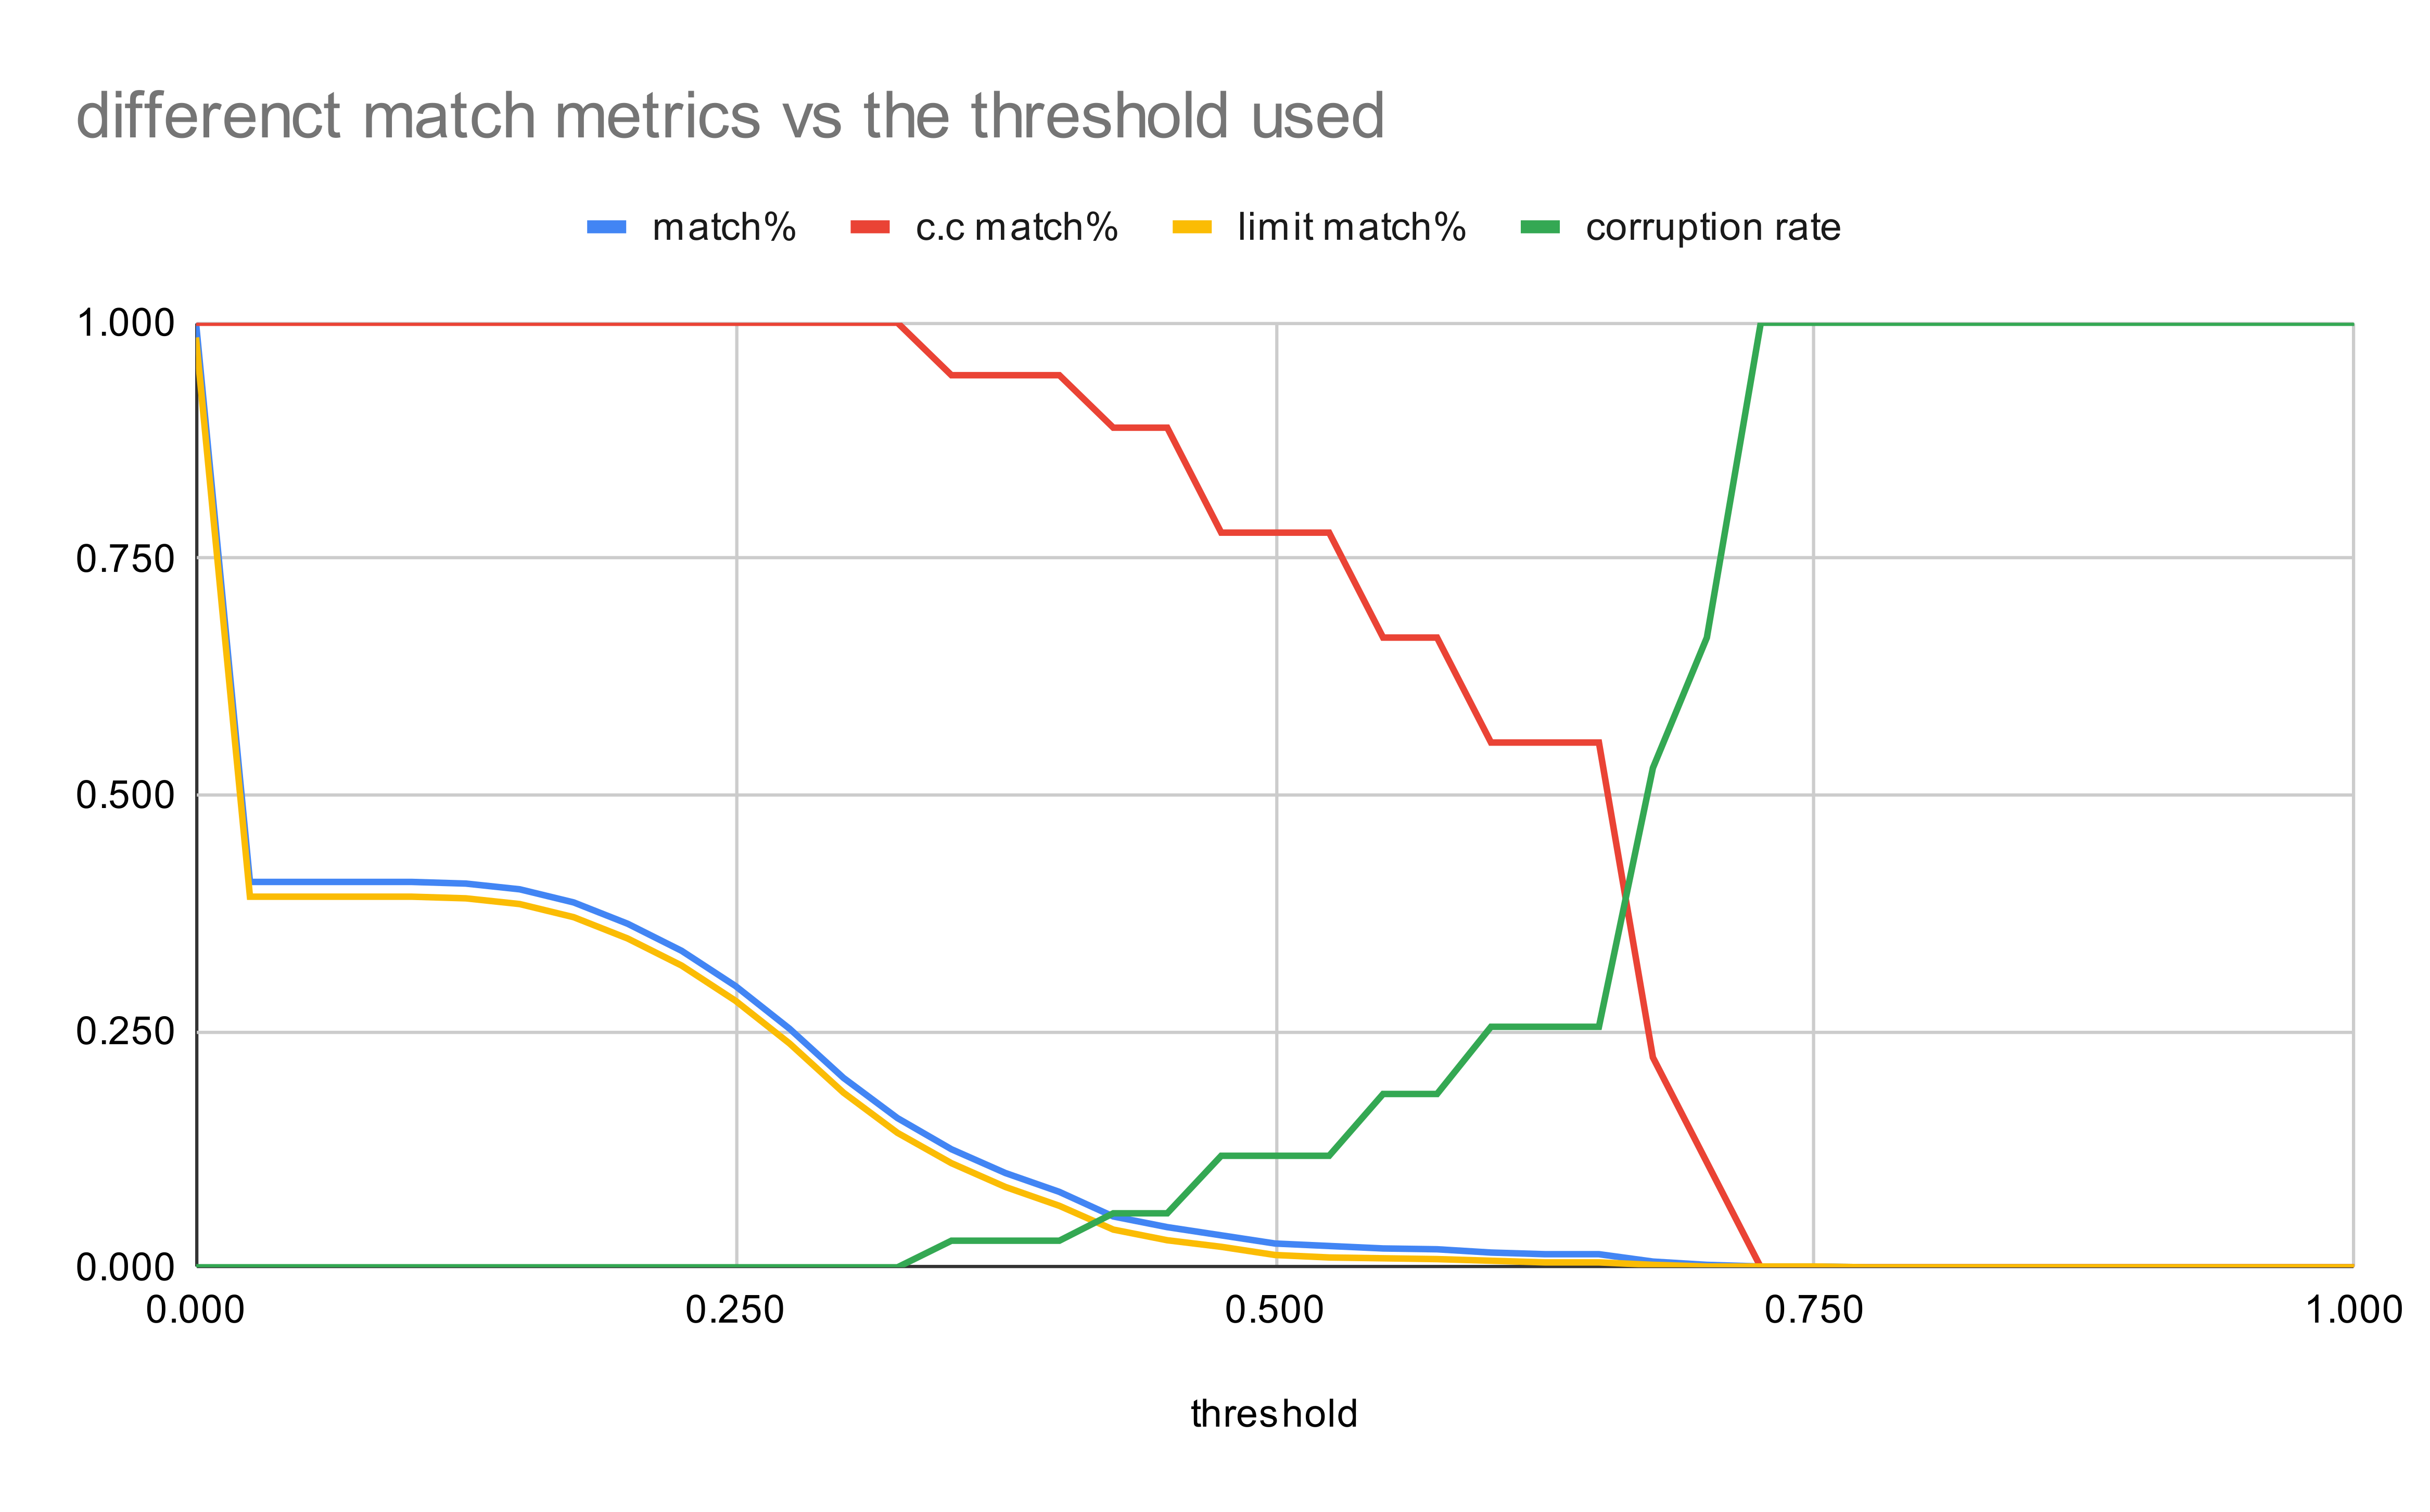
\includegraphics[height=0.5\textwidth]{pictures/match_metrics_vs_threshold_used.png}
\end{figure}

Now, let's consider the graph connection Laplacian algorithm of \cref{document:GCL} tasked with solving a 500-piece puzzle
using our Comparator of \cref{document:my_comparator}.
A threshold of 0.425 is chosen;
This implies a limit match\% of 0.04 and a corruption rate of 0.057.
What would this mean in terms of accuracy of the results?

\subsubsection{Definitions}\label{document:proof_definitions}
This set of definitions are useful to better understand the next section:

\begin{itemize}
  \item \textbf{Connection:}\newline
  When two sides of two different pieces are joined they form a connection.
  A solved puzzle with \(N\) pieces, (assuming it is squared) has around \(2N\) total connections.

  \item \textbf{Possible Combinations:}\newline
  A puzzle with N pieces can be put together in many different ways,
  (Even if not all of 	them actually fit together).
  The total number of possible combinations is \(N! \times 4^N\) where
  \(N!\) represent all possible way to combine the pieces in a particular position, and
  \(4^N\) represents all possible orientations that each piece can have.
  \item \textbf{Possible Correct Combination:}\newline
  Is one of the possible combinations where all the connections are considered a match
  by the comparing algorithm.
  \item \textbf{Actual Correct Combination:}\newline
  An Actual Correct Combination is a Possible Combination that
  is also the correct solution of the original puzzle	
\end{itemize}

\subsubsection{Corruption Rate Analysis}
\begin{figure}[H]
  \caption{Neighbors comparison vs Corruption rate of graph connection laplacian algorithm of \cref{document:GCL}. Image taken from paper~\cite{GCL} page 34.}\label{fig:GCL_Corruption_Rate}
  \centering
  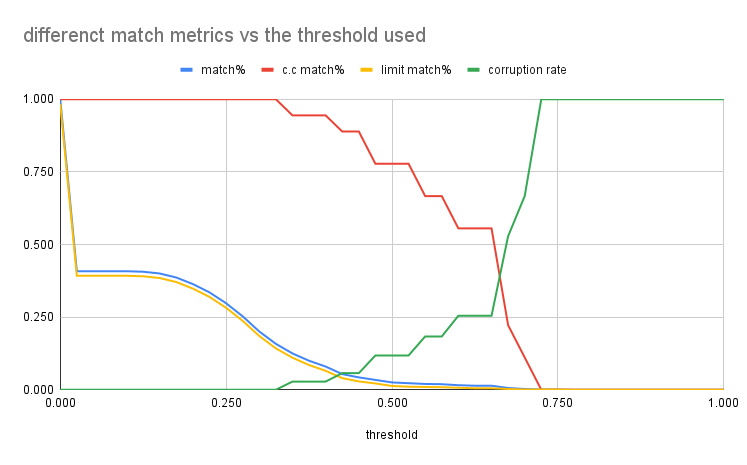
\includegraphics[height=0.35\textwidth]{pictures/corruption_rate.png}
\end{figure}

In \cref{fig:GCL_Corruption_Rate}, it can be observed that at a corruption rate of 0.057,
a neighbors comparison metric of roughly 80\% can be anticipated.
This implies that, on average, one out of every five connections will be incorrect.
In the context of a puzzle comprising 500 pieces (equating to approximately 1000 connections),
an estimated 200 connections will be inaccurate on average.
It is reasonable to assert that this outcome is suboptimal.

\subsubsection{Limit Match\% Analysis}
Let's remember that \(limit\_match\% = 0.04\).

Given that in a puzzle with N pieces there are around \(2N \) connections,
the probability of one random combination to be a
possible correct combination is: \(0.04^{2N}\).

The total number of possible combinations are \(N! \times 4^N\),
which means that on average, in a puzzle with \(N\) pieces,
there will be \(0.04^{2N} \times N! \times 4^N \)
possible correct combinations.

For \( N = 500 \) the expected number of possible combinations is around \( 1.5 \times 10^{37} \).
Which makes the chance of finding the actual correct combination basically zero.
\subsubsection{Conclusion}
In this case both the match\% and the corruption rate are bad enough to make a correct reconstruction impossible.
To lower limit match\% is necessary to increase the threshold, but this would increase the corruption rate.
To lower the corruption rate is necessary to decrease the threshold, but this would increase the limit match\%.
This means that, regardless of the threshold chosen, our comparison algorithm \cref{document:my_comparator}
can not work with a state of the art solver \cref{document:GCL}.


\subsection{Future Works}

Until now this paper has not painted a positive picture about real-world
puzzle solving. The current digital puzzle solver achieves a good time
complexity, but requires really precise input data that we didn't manage
to achieve with our real-world comparator (\cref{document:my_comparator}).
On the other hand we managed to create a Solver (\cref{document:my_solver})
that could operate with the noisy data generated by our comparator;
But the greater reliability came at the expense of time complexity,
and this meant that the maximum size of puzzle that could be solved was limited.

Despite this inconvenience we think there is still a chance to solve
the problem by significantly improving the comparator.

\subsubsection{Machine Learning Based Comparator}

Some minor improvements to the comparator can be made by spending some time
tweaking the current algorithm.
However, it is clear that for a task of this nature,
the most viable solution would likely involve
leveraging machine-learning techniques.

But this presents a significant challenge: manually testing if certain
pieces fit together, followed by scanning and labeling them,
is a time-intensive process that could require hundreds,
if not thousands, of hours.

However we just created a puzzle solver that, even with a suboptimal
time complexity, can easily solve small size real world puzzles.
We could use it to solve a couple hundred small size puzzles,
and automatically label the results for us,
paving the way to a superior machine learning based comparator.

\subsubsection{Labeling tool}

To facilitate ours or someone else's future attempt to create a 
machine-learning-based comparator;
We added to our program the capability to export the data useful
to train a machine learning model.
This section will explain the format of the data.

\paragraph{Basic notions}

One piece is uniquely identified by his id \texttt{piece\_id}.
The id is an integer that goes from 0 to \mbox{Number of pieces - 1}.
Each piece has 4 sides that can be identified by the side \texttt{side\_id},
an integer that goes from 0 to 3.

\paragraph{Image of each piece}

Inside the folder \texttt{results/pieces} the program will generate one image
for each one of the pieces of the puzzle. The file will be named \texttt{\{piece\_id\}.jpeg}.
An example can be seen in \cref{fig:result_pieces}

\begin{figure}[H]
  \caption{}\label{fig:result_pieces}
  \centering
  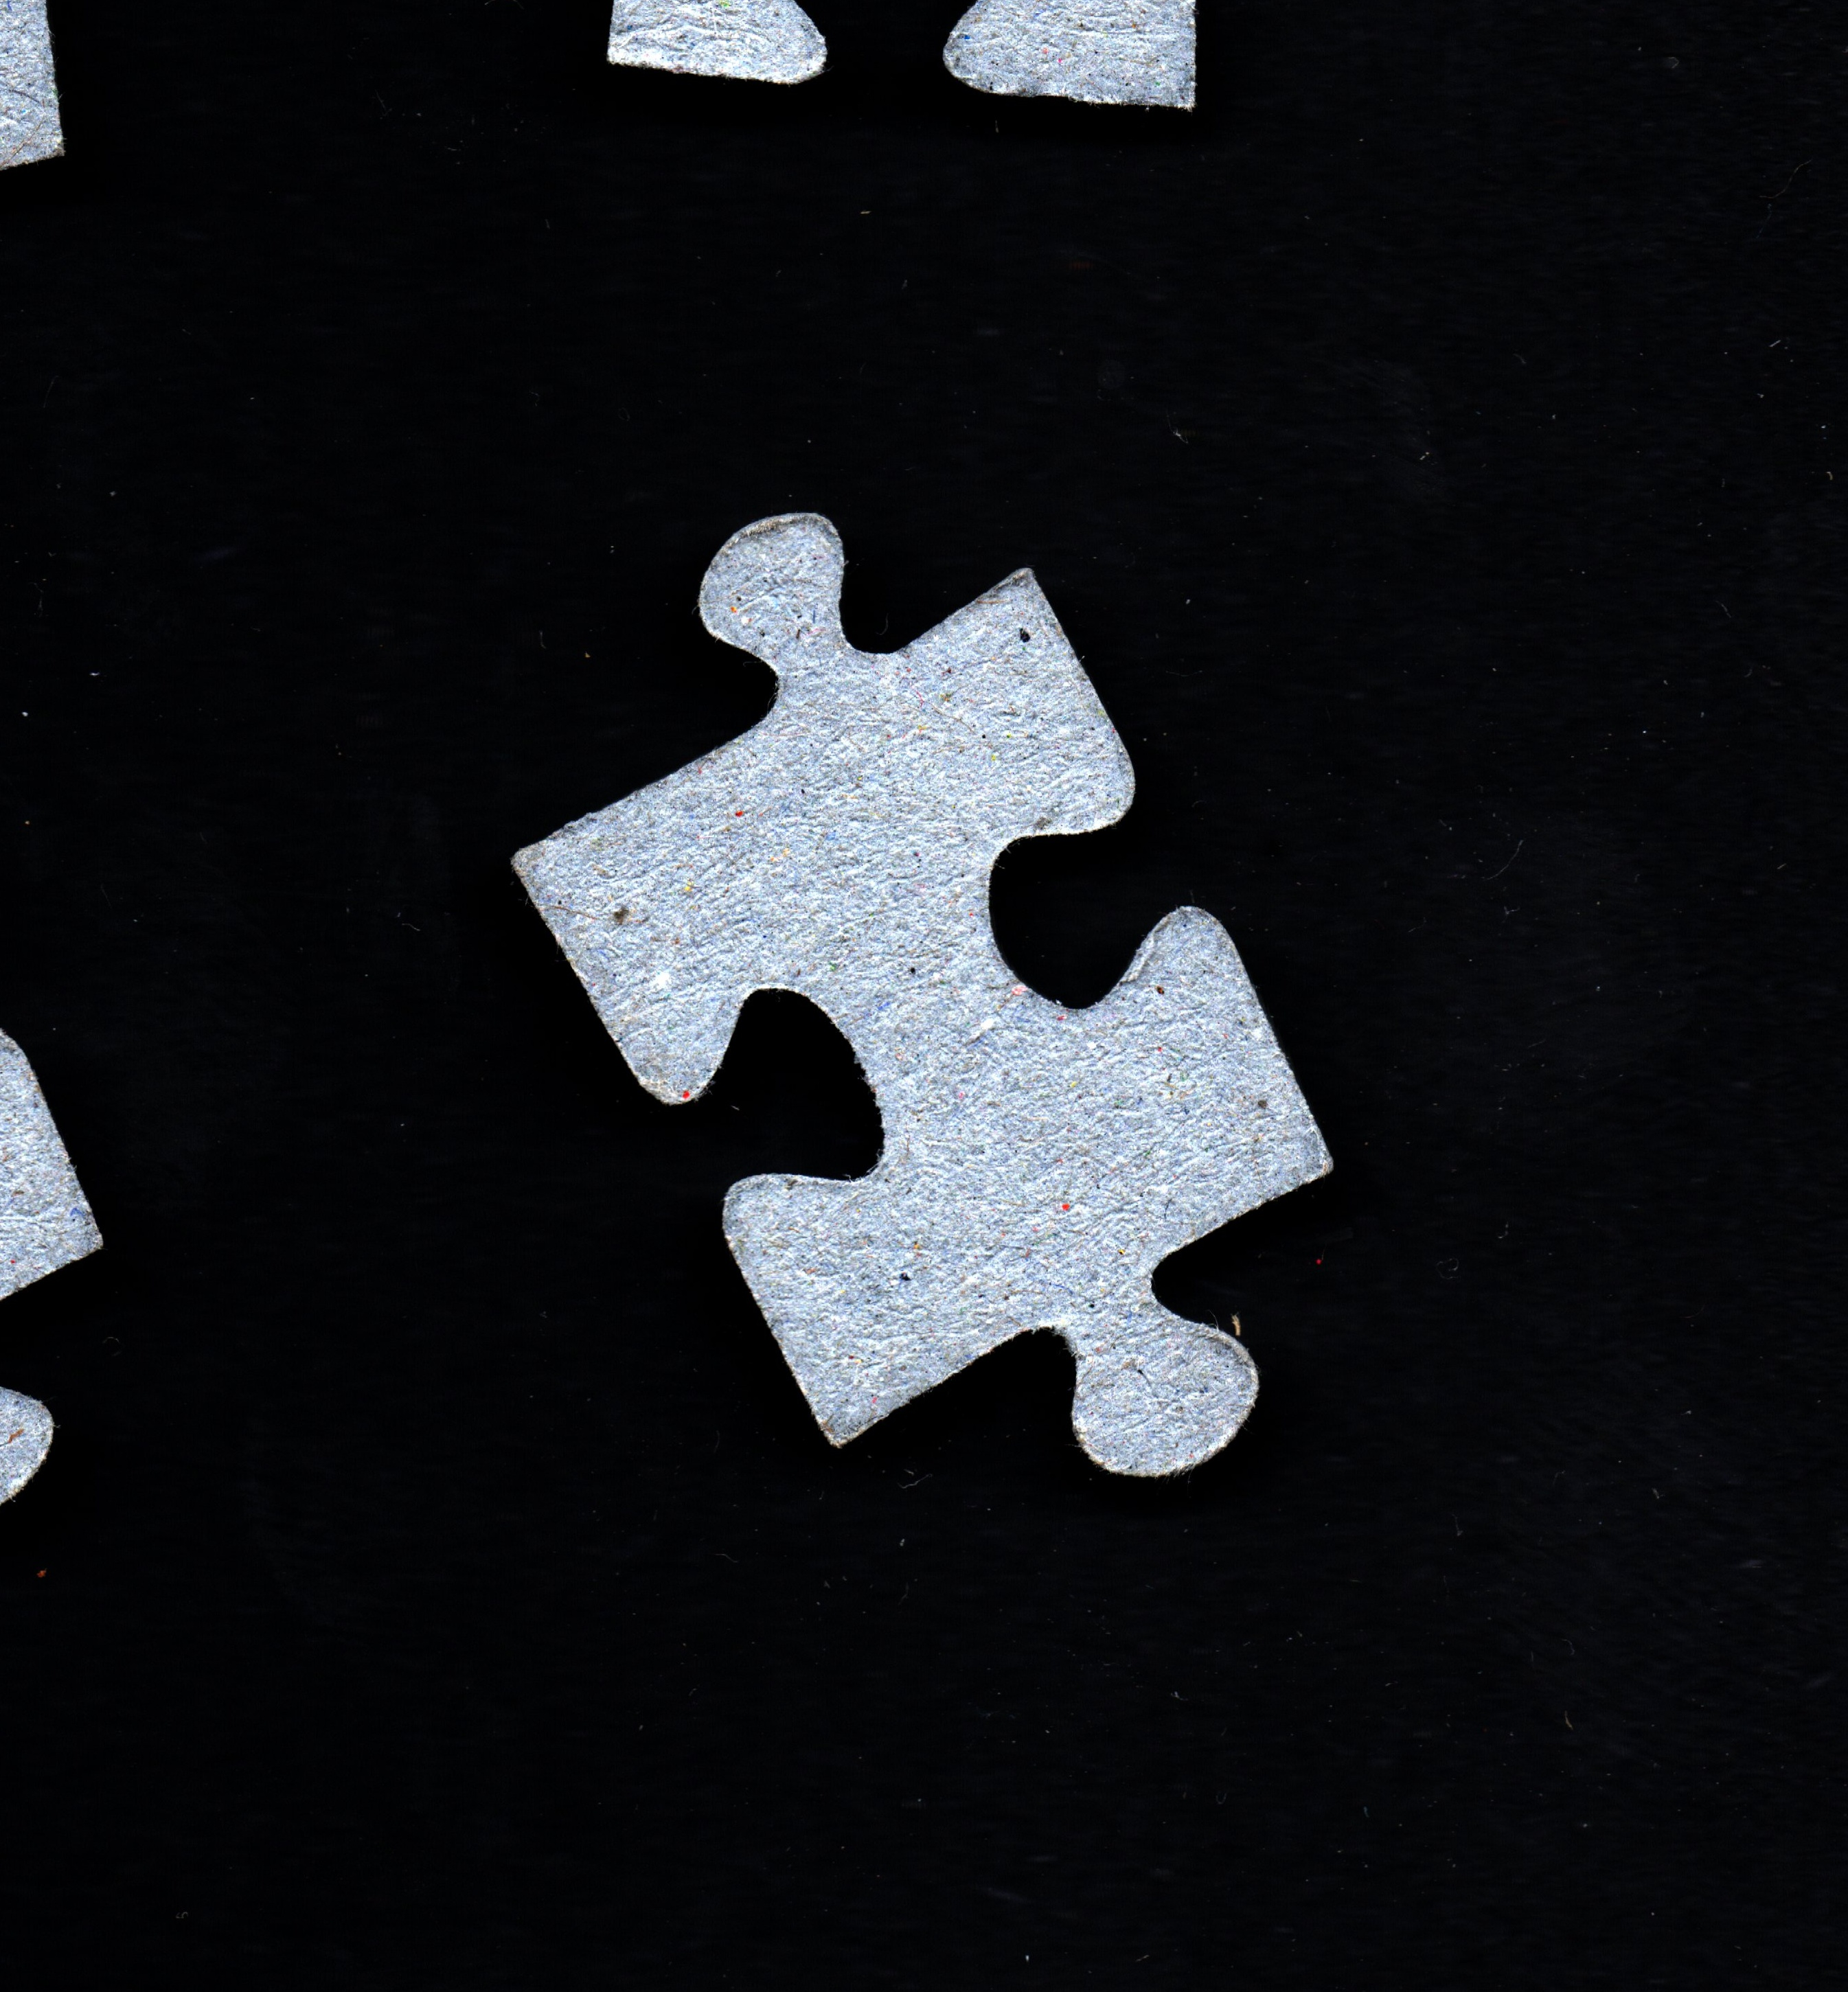
\includegraphics[height=0.3\textwidth]{pictures/result_pieces.jpeg}
\end{figure}

\paragraph{Image of each side}

Inside the folder \texttt{results/sides} the program will generate one image 
for each side of each piece. The images will be named \texttt{\{piece\_id\}\_\{side\_id\}.jpeg}.
An example can be seen in \cref{fig:result_sides}

\begin{figure}[H]
  \caption{}\label{fig:result_sides}
  \centering
  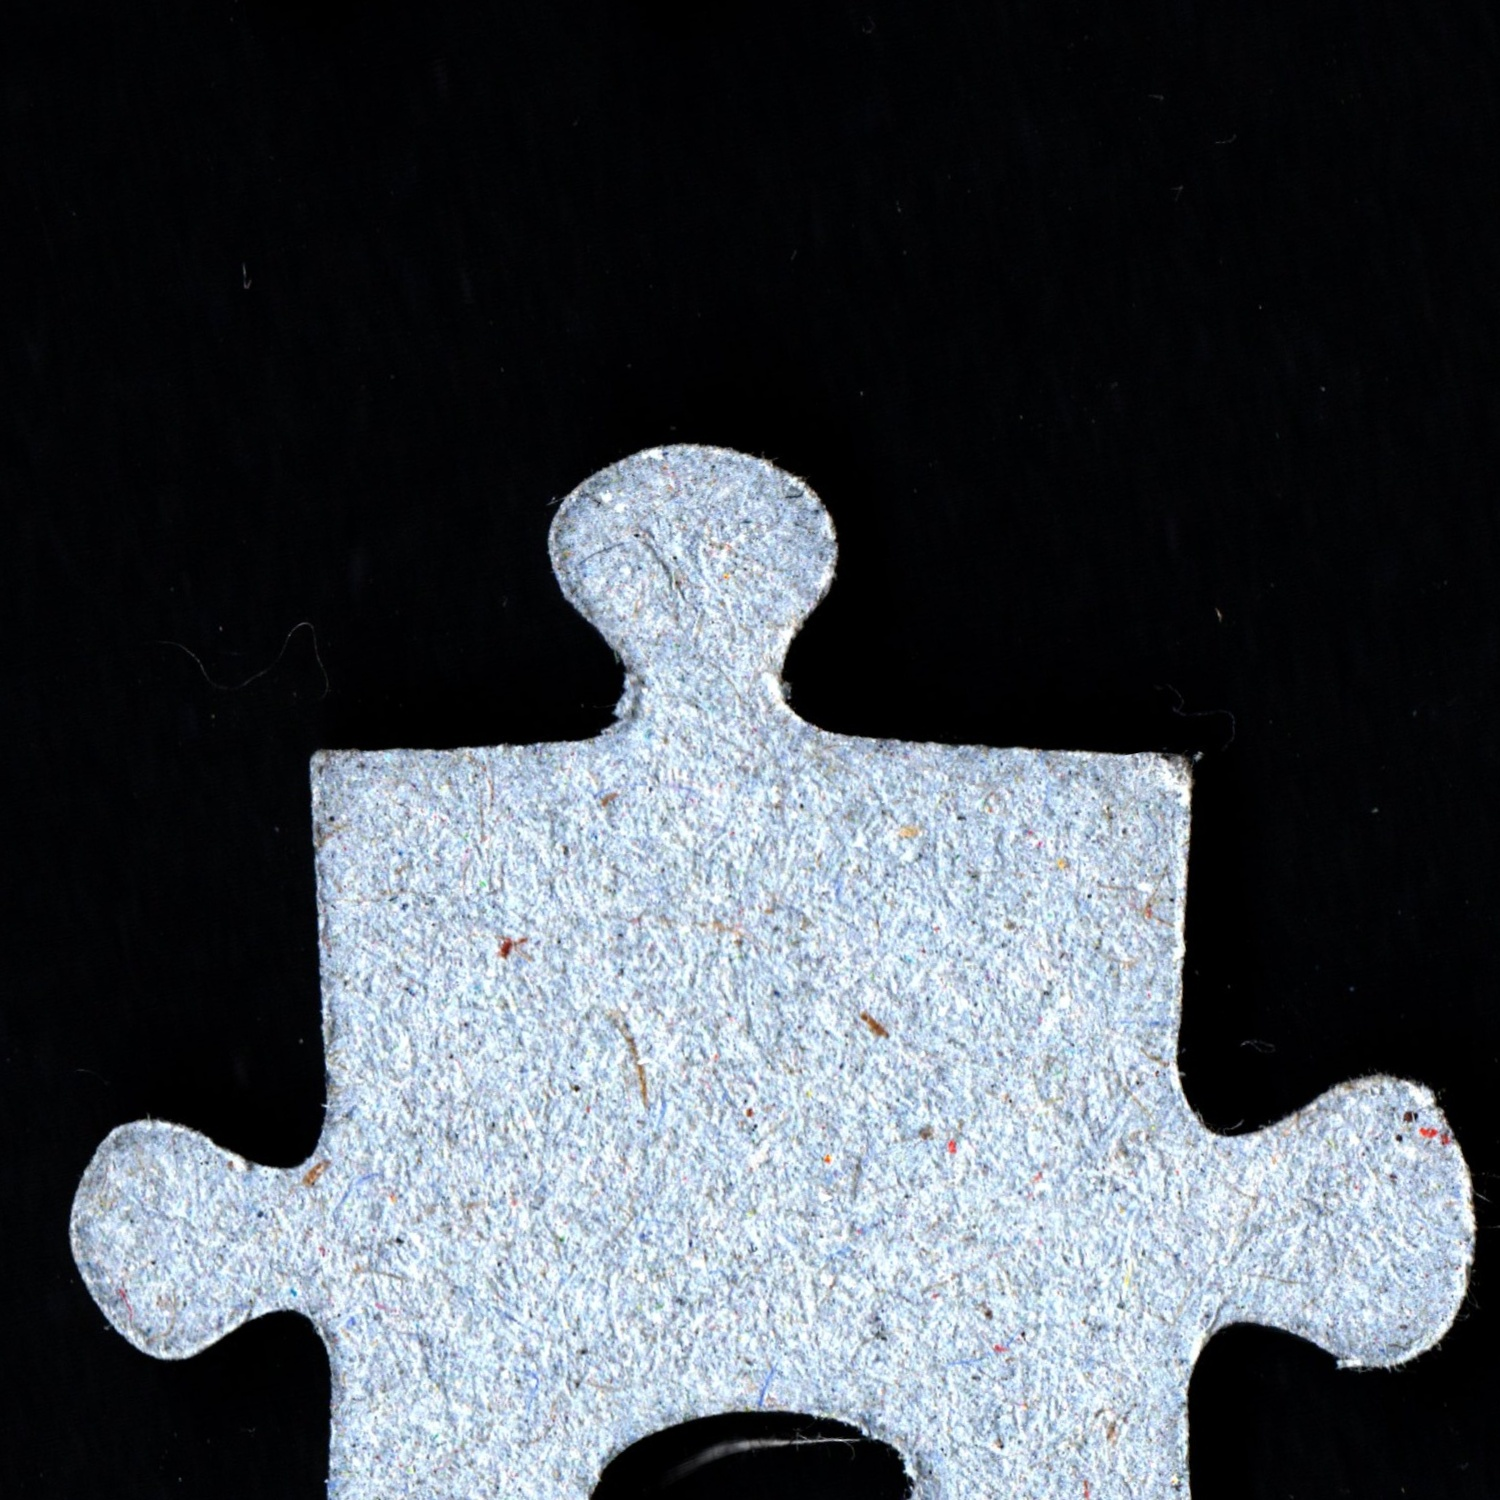
\includegraphics[height=0.3\textwidth]{pictures/result_sides.jpeg}
\end{figure}

\paragraph{Corners of each piece}
The file \texttt{corners.json} will be generated inside the folder \texttt{results}.
This file will contain a list of pieces.
Each piece has 4 sides, and each side has the coordinates of the two points
that delimit itself.\newline
An example of the generated json can be seen below.


\begin{minipage}{\textwidth}
  \begin{lstlisting}
    [
      {
        "piece_id": 0,
        "side_0": {
          "p1": {"x":955, "y":1924},
          "p2": {"x":1024, "y":1016}
        },
        "side_1": {
          "p1": {"x":1024, "y":1016},
          "p2": {"x":1850, "y":1028}
        },
        "side_2": {
          "p1": {"x":1850, "y":1028},
          "p2": {"x":1814, "y":1992}
        },
        "side_3": {
          "p1": {"x":1814, "y":1992},
          "p2": {"x":955, "y":1924}
        }
      },
      {...},
      {...},
      ...
    ]
  \end{lstlisting}
\end{minipage}

\paragraph{Match for each side}
The file \texttt{connections\_result.json} will be generated
inside the folder \texttt{results}. This file will contain a list of pieces,
each piece has 4 sides, and each side has a link to the side of the piece
that matches it. The link can be null if the side is along the border.\newline
An example of the generated json can be seen below.


\begin{minipage}{\textwidth}
  \begin{lstlisting}
    [
      {
        "piece_id": 12,
        "side_0": {
            "piece": 5,
            "side": 0
        },
        "side_1": {
            "piece": 8,
            "side": 0
        },
        "side_2": {
            "piece": 0,
            "side": 0
        },
        "side_3": null
      },
      {...},
      {...},
      ...
    ]
  
  \end{lstlisting}
\end{minipage}

\subsection{Conclusion}

In conclusion, this paper has successfully achieved its objectives.
It has provided a comprehensive explanation of why real-world puzzles
present greater challenges compared to their digital counterparts.
Additionally, it has been shown that the same algorithm can have drastically worse
performance when working with real-world puzzles compared to digital ones.

Furthermore, we have developed a highly effective labeling tool,
which holds great promise for future applications in creating a
machine-learning-based comparator. Such a comparator has the potential
to greatly facilitate puzzle-solving algorithms by providing more
accurate data.

Even the solver we have created can be considered a success.
While its time complexity may be less favorable when compared to state-of-the-art
digital puzzle solvers, it stands as a strong contender in the realm of
real-world puzzle-solving algorithms. In fact, it may even be considered
one of the best available online for tackling real-world puzzles.

All the code used in this project is available on the GitHub repository: \url{https://github.com/lucaSartore/PuzzleSolver}.

\begin{figure}[h]
  \caption{example of a result render of a digital puzzle}\label{fig:result_digital}
  \centering
  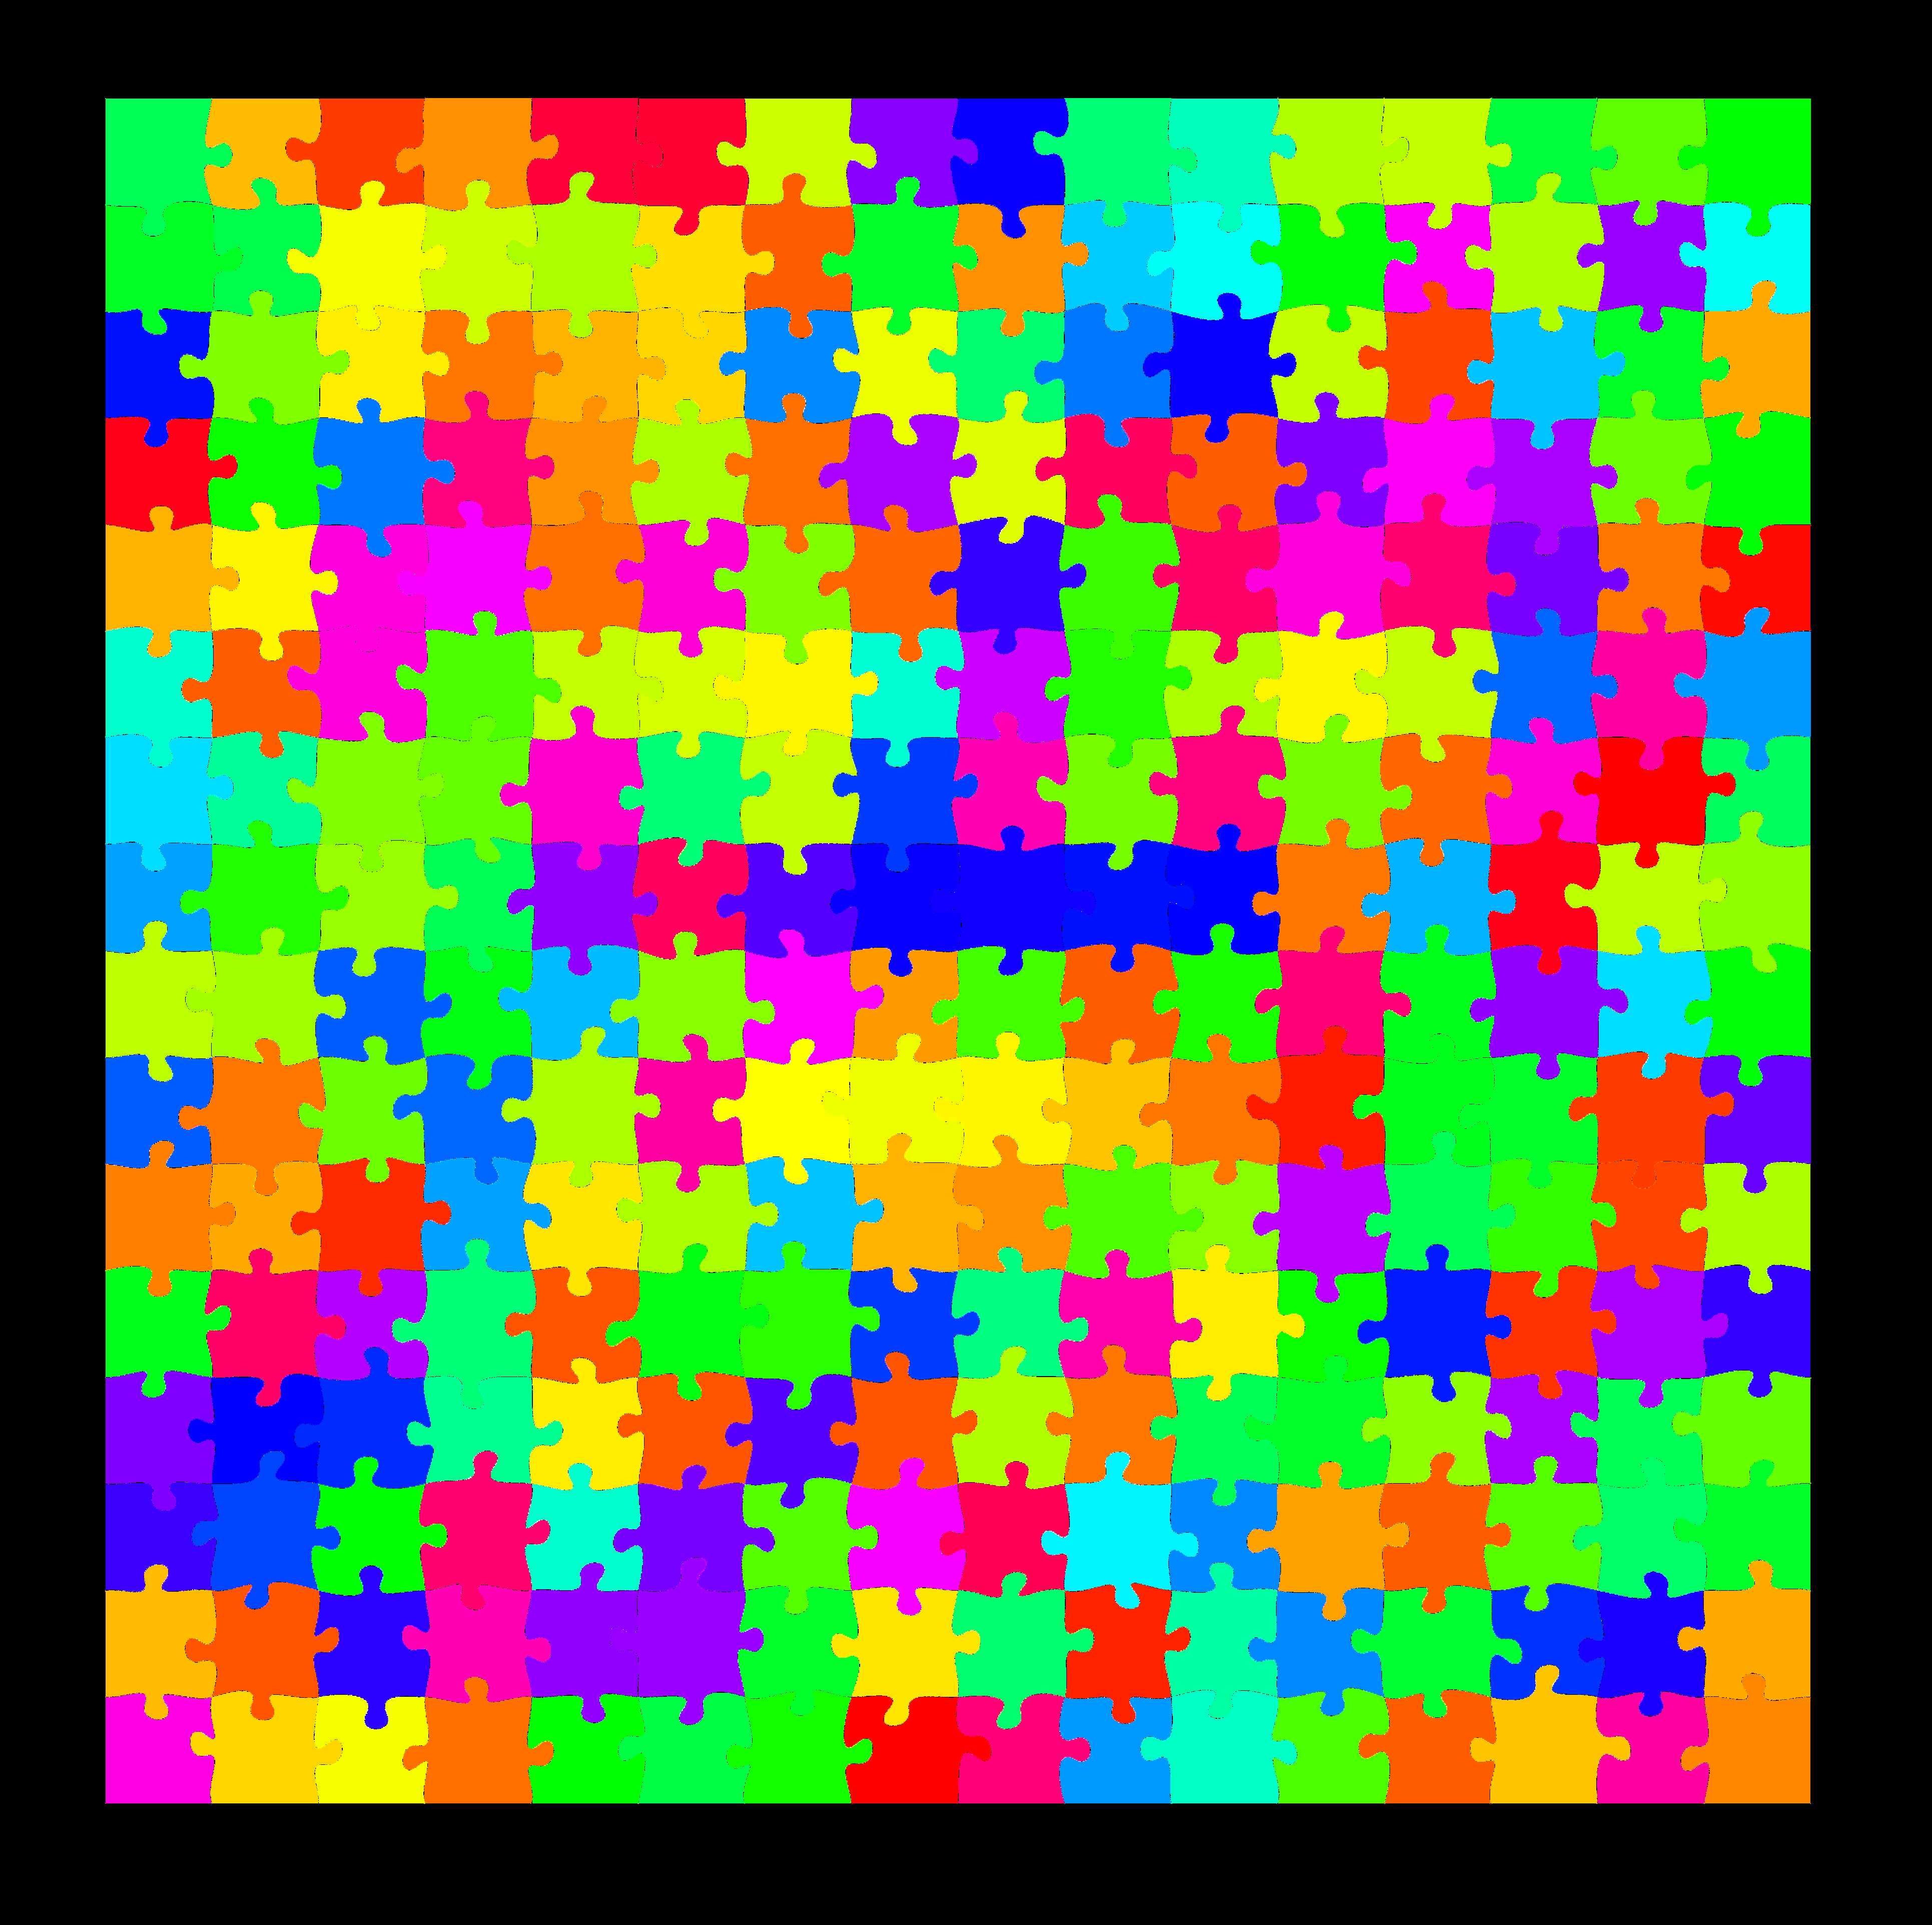
\includegraphics[height=0.6\textwidth]{pictures/result_digital.png}
\end{figure}

\begin{figure}[h]
  \caption{example of a result render of a real world puzzle}\label{fig:result_real}
  \centering
  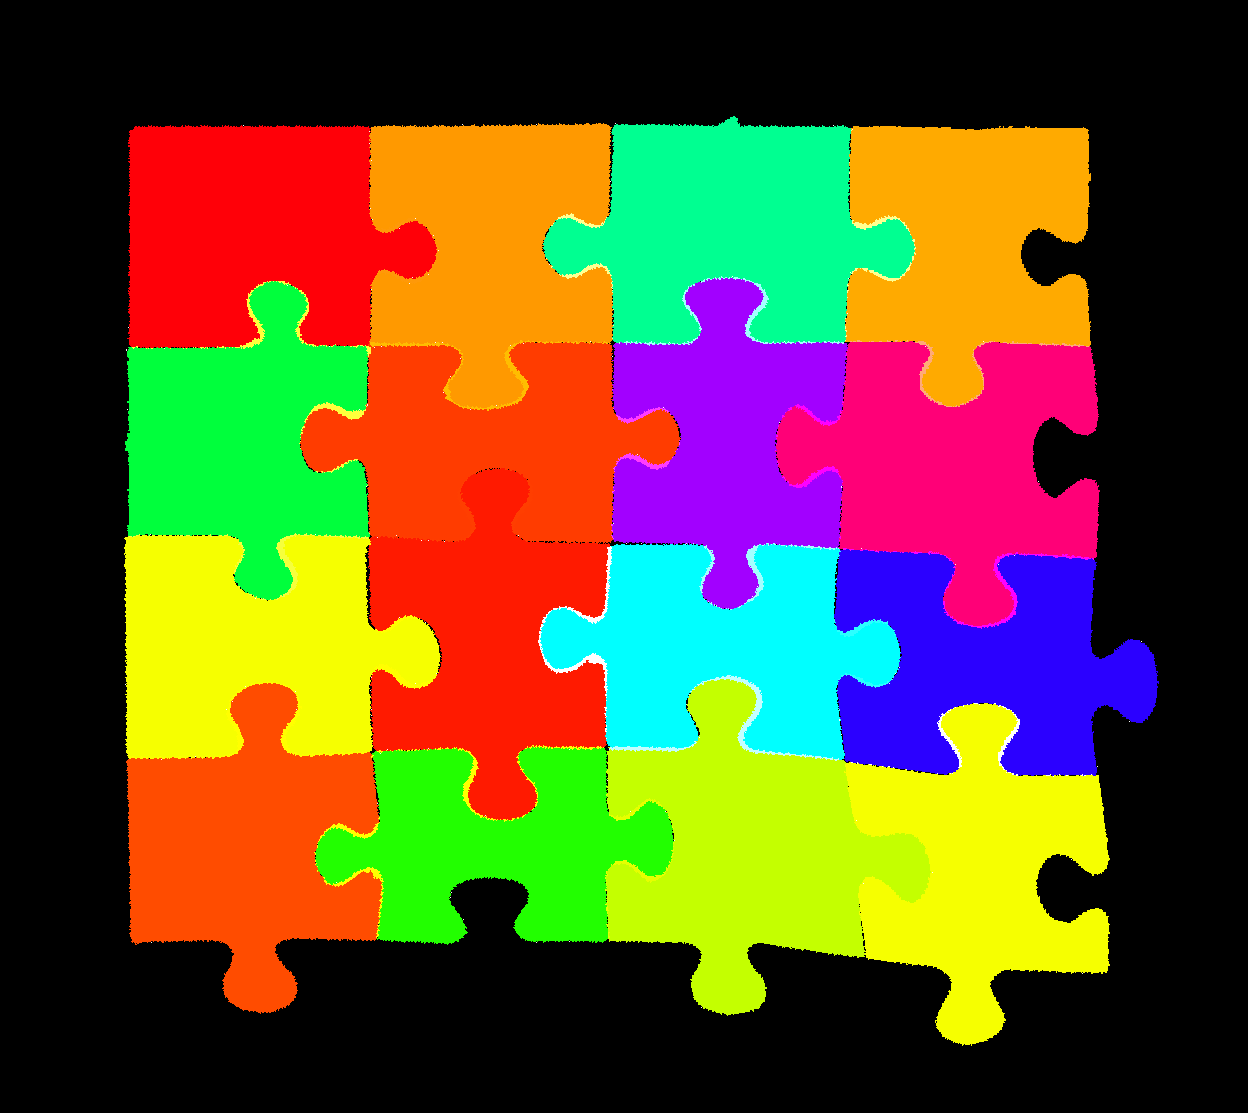
\includegraphics[height=0.6\textwidth]{pictures/result_real.png}
\end{figure}

% referneces page
\clearpage
\begin{thebibliography}{9}

  %Graph Connection Laplacian
  \bibitem{GCL}
    Vahan Huroyan, Gilad   Lerman and Hau-Tieng Wu,
    Solving Jigsaw Puzzles By The Graph Connection Laplacian,
    2020.
    \url{https://arxiv.org/pdf/1811.03188.pdf}.
  % Genetic algorighm
  \bibitem{GA}
    Dror Sholomon, Omid David and Nathan S. Netanyahu,
    A Genetic Algorithm-Based Solver for Very Large Jigsaw Puzzles,
    2013.
    \url{https://openaccess.thecvf.com/content_cvpr_2013/papers/Sholomon_A_Genetic_Algorithm-Based_2013_CVPR_paper.pdf}.
  
    % Claim of best solution O(N^2)
  \bibitem{ON2Claim}
    Michael Brand,
    No easy puzzles: Hardness results for jigsaw puzzles,
    2015.
    \url{https://www.sciencedirect.com/science/article/pii/S0304397515001607}.

    % abtosoftware real world solution
  \bibitem{Abto}
    AbtoSoftware,
    Computer Vision Powers Automatic Jigsaw Puzzle Solver,
    2019.
    \url{https://www.abtosoftware.com/blog/computer-vision-powers-automatic-jigsaw-puzzle-solver}.
  
\end{thebibliography}

\end{document}
